% !TEX program = xelatex
\documentclass[12pt,a4paper]{ctexart}

% ===== 页面布局（上下 2.54cm、左右 3.18cm） =====
\usepackage[top=2.54cm,bottom=2.54cm,left=3.18cm,right=3.18cm]{geometry}
\usepackage{setspace}
\linespread{1.4}

% ===== 字体 =====
% 特殊符号（★△✓∈）归入 CJK 类经中文字体回退；其中 ✓ 各中文字体均缺字形，
% 经 xeCJK 子分区机制单独路由到 Segoe UI Symbol（font_test4.tex 验证 0 缺字形）
\xeCJKDeclareCharClass{CJK}{"2605, "25B3, "2713, "2208}
\xeCJKDeclareSubCJKBlock{SYM}{"2713 -> "2713}
\setCJKmainfont{SimSun}[AutoFakeBold=2.5, SYM=Segoe UI Symbol]
\setCJKsansfont{SimHei}
\setCJKmonofont{SimSun}[SYM=Segoe UI Symbol]
\setmonofont{Consolas}[Scale=0.82]  % 附录代码等宽字体；中文注释经 \setCJKmonofont{SimSun} 回退显示

% ===== 标题编号（一级"一、"黑体三号居中，二级"（一）"黑体四号） =====
\ctexset{
  section = {
    format = \zihao{3}\heiti\centering,
    name = {,、},
    number = \chinese{section},
    aftername = \quad
  },
  subsection = {
    format = \zihao{4}\heiti,
    name = {（,）},
    number = \chinese{subsection},
    aftername = \quad
  },
  subsubsection = {
    format = \zihao{-4}\heiti,
    number = \arabic{subsubsection},
    aftername = \quad
  }
}

% ===== 宏包 =====
\usepackage{amsmath,amssymb}
\usepackage{booktabs}
\usepackage{graphicx}
\usepackage{float}
\usepackage{caption}
\usepackage{enumitem}
\usepackage{multirow}
\usepackage{fancyhdr}
\usepackage{fvextra}
\usepackage{verbatim}

% ===== 页脚居中页码、无页眉（官方：页码页脚中部，摘要页起编 1） =====
\pagestyle{plain}
\renewcommand{\headrulewidth}{0pt}

% ===== 图表标题五号宋体 =====
\captionsetup{font=small,labelsep=quad}

% ===== 附录代码直引（VerbatimInput 等效 lstinputlisting，保证与实际代码逐行一致） =====
% 注：breaklines/breakanywhere 属 fvextra 扩展（fancyvrb 原生不支持），必须用 fvextra 承载
\fvset{frame=single,numbers=left,numbersep=6pt,fontsize=\zihao{-5},
       baselinestretch=1.05,tabsize=4,breaklines=true,breakanywhere=true}

\begin{document}

% ============================================================
% 摘要专用页（官方：电子版第一页，仅标题+摘要+关键词，≤1 页）
% ============================================================
\begin{titlepage}
\centering
{\zihao{3}\heiti 红色警戒——战略节点攻防与撤退调度规划\par}
\vspace{0.5cm}
{\zihao{4}\heiti 摘\hspace{2em}要\par}
\vspace{0.2cm}

\begin{minipage}{0.95\textwidth}
\zihao{-4}
\setlength{\parindent}{2em}
本文围绕苏军与盟军在 436 节点、603 通路战场网络上的攻防对抗，建立部署、补给与攻防转移三类优化模型。先对附件做几何核验与图结构分析，确认坐标单位为千米，并识别出 8 条跨阵营前线咽喉边与苏军 23 节点孤立后方分量，为建模提供结构依据。

针对问题一，构建覆盖型广义指派整数规划模型，以加权火力覆盖—生存—指挥通信综合效能为目标，用分支定界法求解双方部署与指挥节点选址。苏军最优指挥节点为 136（综合效能 0.7688），盟军为 384（综合效能 0.7732），求解器 MIPGap 均为 0，证明全局最优；权重 $\pm 20\%$ 扰动及直射距离、防空半径、空中上限的参数扫描下指挥节点翻转数为 0，方案稳健。

针对问题二，建立运输、护航、破交损失、人力四类成本分层的补给网络优化模型，以 McCormick 线性化求解 0-1 护航规划，并用 Stackelberg 博弈刻画破交—护航对抗。基线情形下苏军后勤总成本 109614 元/日、盟军 145773 元/日，破交损失占比最高（苏军 68.8\%、盟军 67.1\%）；对抗最坏情形下成本分别上升 50.83\% 与 48.94\%（含人力 $\mathrm{TC}_{total}$ 主口径）；蒙特卡洛仿真验证解析期望损失，偏差仅 0.72\% 与 1.54\%。

针对问题三，以贪心构造加 Lanchester 蒙特卡洛评估设计苏军进攻方案，主攻方向为 55$\to$372 边，7 节点夺控序列平均攻方剩余兵力比 0.8862、各步胜率不低于 0.98；盟军战略转移以人员为决策量纲，在通信畅通与通信中断两情景下整体人员生存概率分别为 0.7956 与 0.6730，差 0.1226，量化揭示了通信的生存价值。

\vspace{0.3cm}
\noindent{\heiti 关键词：}整数规划；Stackelberg博弈；Lanchester平方律；蒙特卡洛仿真；灵敏度分析
\end{minipage}
\end{titlepage}

% ============================================================
% 一、问题重述
% ============================================================
\section{问题重述}

在《红色警戒》的平行世界设定中，苏军与盟军在一张由 436 个作战节点与 603 条通路构成的战场网络上展开争夺\cite{ref1}。双方只能在本方颜色相同的初始区域内部署兵力，每个节点带有 0 到 1 之间的防御强度。

双方兵力与装备如下：苏军有动员兵 125 万人、侦察机 500 架、天启重型坦克 180 辆、犀牛主战坦克 300 辆、猎犬轻型战车 420 辆、V3 远程火箭车 7000 辆；盟军有动员兵 100 万人、侦察机 300 架、光棱重型坦克 340 辆、幻影中型坦克 570 辆、灰熊轻型坦克 800 辆、光棱自行火炮 14000 辆。每方可设置 10 个防空炮阵地据点，空中单位（战略空袭单位）不宜部署过多。装备的重量、速度、行程、射程等参数由附件二给出。需要研究三个问题。

\textbf{问题一}：综合考虑节点防御强度、沿路网的机动距离、武器射程（坦克直射距离、自行火炮最大射程）与防空阵地覆盖半径，确定双方各类型作战单位（动员兵、轻/中/重型坦克、自行火炮、防空炮阵地）的部署节点与数量，并为双方各选定一个最优前线指挥节点（可驻扎任一己方节点）与 3 个备选指挥节点，兼顾指挥通信距离、节点隐蔽性与抗毁能力。

\textbf{问题二}：基于问题一的部署结果，为双方分别建立维修包（备件/工具）、弹药与能源（燃油/电池）三类补给的分配与供应优化模型，充分考虑敌方破交与拦截策略，预留规避或护航措施；计算完全不进行补给的消耗模式下维持前线作战所需的总后勤工人数与运输车辆总数；以表格或图形给出最优补给方案，包括配送路径、发车周期、每车装载量等信息。

\textbf{问题三}：设定苏军为进攻方、盟军为防守方。其一，设计苏军进攻计划，包括主攻方向、优先攻占的节点序列与各突击梯队（坦克/步兵/火炮配比）的兵力编成；其二，盟军需收缩至后方安全节点 352、144、149，分别给出通信畅通时的整体转移路线与兵力收拢计划（含殿后部队），以及通信中断时各部队按独立预案分散转移的方案，并对比两种情况下盟军部队的整体生存概率差异。

题目涉及若干军事术语，且两个附件各有特定内容，为便于阅读，先给出名词解释与附件说明，见表~\ref{tab:terms}。

\begin{table}[H]
\centering
\caption{名词解释与附件说明}
\label{tab:terms}
\zihao{5}
\begin{tabular}{p{2.8cm}p{10.8cm}}
\toprule
名词/附件 & 说明 \\
\midrule
破交/拦截 & 攻击方对敌方补给线实施打击以截获物资的作战行动，本文以路径拦截概率度量 \\
前线咽喉边 & 连接两个阵营区域的跨阵营通路，是地面兵力越界的唯一通道 \\
坦克直射距离 & 坦克炮直瞄射击的有效距离，附件二未提供，由假设 A-02 补足 \\
防空覆盖半径 & 防空炮阵地对空中威胁的防护范围，覆盖内部署单位生存率提升，由假设 A-03 补足 \\
梯队编成 & 进攻部队按坦克、步兵、火炮等兵种比例编组的作战单元 \\
殿后部队 & 转移行动中留守迟滞敌方追击、掩护主力撤退的部队 \\
消耗模式 & 完全不进行补给、仅靠初始携行物资维持作战的后勤模式 \\
附件一 & 作战节点与通路数据：436 个节点（编号、坐标、阵营、防御强度）与 603 条通路（端点、长度 km） \\
附件二 & 红警装备参数表：双方 8 型装备的重量、武器、速度、行程、射程等参数 \\
\bottomrule
\end{tabular}
\end{table}

% ============================================================
% 二、问题分析
% ============================================================
\section{问题分析}

\subsection{兵力部署与指挥节点选址的结构特征分析}

问题一要求同时决定六类单位在数百个节点上的部署数量与指挥节点位置，属于覆盖型广义指派问题，是 NP-hard 的组合优化\cite{ref3,ref4}。核心难点有三：一是决策变量为整数且规模大（单位类型 $\times$ 己方节点数达数千）；二是火力覆盖存在重复覆盖时的边际递减效应，直接按覆盖次数求和会高估效能；三是指挥节点选址与部署方案相互耦合，同一节点在不同部署下的优劣可能不同。拟采用线性化手段将模型化为纯线性混合整数规划（MIP），用分支定界法证明全局最优；指挥节点采用多准则评分生成候选、逐候选重解部署 MIP 的枚举策略。附件数据的图结构（咽喉边、孤立分量）将直接转化为模型约束，详见第~\ref{sec:global}~节。

\subsection{补给线对抗下的成本优化思路}

问题二的补给需求由问题一的部署结果派生，形成两问之间的数据接口。难点在于护航决策与破交损失的双线性耦合：启用护航能降低损失，但护航本身有成本，二者乘积项使目标非线性。拟将后勤成本分解为运输、护航、破交期望损失、人力四类独立分项，路径集预枚举后用 0-1 规划建模，双线性项以 McCormick 线性化精确处理\cite{ref7}。敌方的破交策略构成对抗：我方先承诺路径与护航组合，敌方观察后将有限破交预算投向收益最大的路径，这是 Stackelberg 博弈结构\cite{ref10}，拟以敌方最优响应下的最坏情形成本量化对抗代价。

\subsection{进攻序列与两情景转移的时序与随机性}

问题三包含两个方向。苏军进攻是多阶段时序决策，战斗损耗使状态转移非线性：动态规划的状态空间随节点数指数爆炸，时序展开 MIP 的松弛很弱，故拟采用贪心构造加 Lanchester 平方律蒙特卡洛评估的混合策略\cite{ref8,ref9}，并讨论替代算法的取舍理由。盟军转移的决策信息结构不同：通信畅通时是单一决策者的全局优化（容量约束分配加最短路），通信中断时退化为各部队的分散独立预案。两情景的生存概率无法解析求得，拟用逐边伯努利拦截的蒙特卡洛仿真各 2000 次估计\cite{ref11}，并对比均值差与分布形态。

% ============================================================
% 三、模型假设
% ============================================================
\section{模型假设}

\begin{enumerate}[label=\textbf{假设\arabic*.},leftmargin=0pt,itemsep=0.4em]
\item \textbf{破交拦截概率与护航效应}。边暴露度按公式 $\mathrm{risk}_e=\min(0.35,\ 0.05+0.10\,\mathbb{I}_{\text{跨阵营}}+0.02\,\min(\deg(a),\deg(b)))$ 计算，护航使该边拦截损失降低 50\%。题目未提供破交数据，公式以边度数与跨阵营属性代理暴露程度，属显式未知参数，参数化形态见表~\ref{tab:paramreg} 的 A-01。
\item \textbf{武器射程与防空覆盖}。坦克直射距离取轻型 1.5 km、中/重型 2.0 km，防空炮阵地覆盖半径 $R_{aa}=3.0$ km，覆盖内部署单位生存率提升 20\%。附件二仅给出自行火炮最大射程（V3 为 16.8 km、光棱火炮为 13.0 km），坦克直射距离与防空半径属题目数据缺口，以假设补足并参数化（表~\ref{tab:paramreg} 的 A-02、A-03）。
\item \textbf{后勤标准参数}。运输车容量 10 吨/车、时速 40 km/h、每车配 2 名司机；单位成本为运输 20 元/km$\cdot$车、护航 500 元/车次、破交损失货值 1000 元/吨、人力 300 元/人$\cdot$日；日消耗率为弹药 0.8 吨/百辆、燃油 0.6 吨/百辆、维修包 0.2 吨/百辆，动员兵按万人折算 0.5 吨/万人（三类合计）。
\item \textbf{战斗损耗规律}。地面交战服从 Lanchester 平方律，单位火力系数取重型 1.0、中型 0.7、轻型 0.3、火炮 0.8、动员兵 0.2、空中 0.5，防御强度以乘性因子 $(1+0.5\,d_n)$ 修正毁伤率；毁伤过程叠加对数正态乘性噪声（$\sigma=0.15$，截断于 $[0.5,1.5]$）。
\item \textbf{守军强度标定}。夺控战斗的守军总量按攻方单步投入的 $k_{def}=0.5+0.3\,d$ 倍标定（$d$ 为节点防御强度），兵种构成为动员兵 45\%、中型 25\%、重型 18\%、火炮 12\%。该线性标定是问题三胜率的关键敏感参数，其局限与影响在第~\ref{sec:err}~节单独讨论。
\item \textbf{距离度量}。火力覆盖判定采用欧氏距离（603 条边的链路长度与坐标欧氏距离比值恒为 1.0000，坐标单位即 km，该简化经几何核验成立）；指挥通信距离采用路网最短路距离（Dijkstra 算法）。
\item \textbf{苏军孤立后方就地防御}。图连通性实测表明战场含 2 个连通分量：主分量 413 节点与苏军后方孤立分量 23 节点。孤立分量与主战场不连通，其内部队无法经路网支援前线，按就地防御部署。
\end{enumerate}

对四项争议假设以显式未知参数的规范形态介入模型，参数登记表见表~\ref{tab:paramreg}，每项含基线值、取值范围（稳定性区间或最坏情形）与模型角色；对应的扫描数据与图见第~\ref{sec:sens}~节。

\begin{table}[H]
\centering
\caption{显式未知参数登记表（A-01 至 A-04）}
\label{tab:paramreg}
\zihao{5}
\resizebox{\textwidth}{!}{
\begin{tabular}{p{2.6cm}p{3.4cm}p{5.6cm}p{3.2cm}}
\toprule
参数 & 基线值 & 取值范围与稳定性 & 模型角色 \\
\midrule
A-01 破交拦截概率 & $\mathrm{risk}_e$ 公式（假设 1） & 对抗最坏情形（含人力 $\mathrm{TC}_{total}$ 主口径）：TC 苏军 $+50.83\%$（109613.7$\to$165334.7 元/日）、盟军 $+48.94\%$（145773.0$\to$217114.0 元/日） & 内生未知参数：静态 $\mathrm{risk}_e$ 基线为主模型输入，Stackelberg 最坏情形为鲁棒性成本量化 \\
A-02 坦克直射距离 & 轻型 1.5 km、中/重型 2.0 km（代表值 $d=2.0$ km） & $d\in[1.0,3.0]$ km 五点扫描，指挥节点翻转数为 0，稳定性区间 $[1.0,3.0]$ km & 外生未知参数（题目数据缺口），经覆盖系数进入 Q1 \\
A-03 防空覆盖半径 & $R_{aa}=3.0$ km & $r\in[2.0,4.0]$ km 五点扫描，防空节点集 Jaccard 相似度恒为 1.0，稳定性区间 $[2.0,4.0]$ km & 外生未知参数（题目数据缺口），经生存加成进入 Q1 \\
A-04 空中部署上限 & $\alpha=10\%$（苏 50 架、盟 30 架） & $\alpha\in[5\%,20\%]$ 四点扫描，指挥节点翻转数为 0，Q2 成本最大传播影响 0.419\% & 题目定性要求（“不宜部署过多”）的定量化 \\
\bottomrule
\end{tabular}
}
\end{table}

\textbf{A-07 粒度选择验证注记}：动员兵以万人为决策粒度（125 万记为 125 单位）属建模粒度选择而非未知参数，目的是避免 $10^6$ 值域造成的整数规划病态。以 0.5 万人更细粒度补做验证算例：双方指挥节点均不翻转，装备部署结构 Jaccard 相似度为 1.0，综合效能 $\varphi$ 最大变化 0.0001，部署结构对粒度稳健。

\textbf{Q2 口径说明}：问题二 MIP 内部目标值（苏军 81690.4、盟军 107511.6 元/日）与重算总成本（109613.7、145773.0 元/日）的差异源于护航成本按固定份额线性化的近似，属计算保真度问题而非未知参数。本文一律以重算可行解的真实总成本 TC 为准，两个口径的差距（相对不含人力成本口径为 7.18\% 与 8.56\%）在误差分析中量化。

% ============================================================
% 四、符号说明
% ============================================================
\section{符号说明}

符号与代码变量名的对照关系在附录代码文件头部以注释形式给出，全部符号见表~\ref{tab:sym}。

\begin{table}[H]
\centering
\caption{符号说明}
\label{tab:sym}
\zihao{5}
\resizebox{\textwidth}{!}{
\begin{tabular}{cll}
\toprule
符号 & 说明 & 单位 \\
\midrule
$x_{c,u,n}$ & 阵营 $c$ 单位类型 $u$ 在节点 $n$ 的部署数量（动员兵以万人计） & 辆/门/万人 \\
$z_c$ & 阵营 $c$ 的前线指挥节点 & 节点编号 \\
$\mathrm{flow}_{c,k,r}$ & 阵营 $c$ 物资 $k$ 经路径 $r$ 的日流量 & 吨/日 \\
$e_r$ & 路径 $r$ 是否启用护航（代码变量 z[r]） & 0-1 \\
$f_r,\ l_r$ & 路径 $r$ 发车频次；每车装载量 & 次/日；吨/车 \\
$\varphi_c$ & 阵营 $c$ 部署综合效能 & 无量纲 \\
$F_c,\ S_c,\ D_c$ & 火力覆盖效能；生存效能；指挥通信距离（部署加权平均路网距离） & 无量纲；无量纲；km \\
$\mathrm{TC}_c$ & 阵营 $c$ 后勤总成本 & 元/日 \\
$P_{surv}$ & 盟军人员生存概率（人员加权） & 0-1 \\
$N_{c,u}$ & 阵营 $c$ 单位类型 $u$ 的总兵力 & 辆/门/万人 \\
$d_n,\ \mathrm{camp}(n)$ & 节点 $n$ 防御强度；所属阵营 & 0-1；-- \\
$L_e$ & 通路 $e$ 长度 & km \\
$R_u$ & 单位 $u$ 武器射程（火炮取最大射程，坦克取直射距离假设） & km \\
$\mathrm{cov}_{u,n,m}$ & 单位 $u$ 在节点 $n$ 能否覆盖敌节点 $m$（射程内为 1） & 0-1 \\
$v_m,\ \mathrm{surv}_u$ & 敌节点 $m$ 目标价值（取 $d_m$）；单位 $u$ 基础生存系数 & 0-1 \\
$R_{aa},\ \mathrm{risk}_e$ & 防空炮阵地覆盖半径；通路 $e$ 破交拦截概率 & km；0-1 \\
$\mathrm{Cap},\ \mathrm{Demand}_{c,k,n}$ & 运输车容量；阵营 $c$ 节点 $n$ 物资 $k$ 日需求 & 吨；吨/日 \\
$w_1,w_2,w_3$ & 问题一目标权重（火力/生存/通信，取 0.5/0.3/0.2） & -- \\
$\lambda_u$ & Lanchester 单位火力系数（代码变量 FIREPOWER） & -- \\
$\alpha$ & 空中单位部署上限比例（A-04，基线 10\%） & -- \\
$\mathcal{T}$ & 盟军战略转移目标节点集 $\{352,144,149\}$ & 节点编号 \\
$C_{trans},C_{escort},C_{loss},C_{labor}$ & 运输、护航、破交损失、人力四类成本 & 元/日 \\
$W_c,\ V_c$ & 阵营 $c$ 总后勤工人数；运输车辆总数 & 人；辆 \\
$D_{max}$ & 主分量路网直径估计（归一化尺度，43.335 km） & km \\
\bottomrule
\end{tabular}
}
\end{table}

算法与求解方法术语见表~\ref{tab:algo}。

\begin{table}[H]
\centering
\caption{算法术语说明}
\label{tab:algo}
\zihao{5}
\begin{tabular}{p{3.6cm}p{10.0cm}}
\toprule
术语 & 说明 \\
\midrule
混合整数规划（MIP） & 决策变量含整数约束的线性优化模型，本文问题一、问题二的求解载体 \\
分支定界法 & MIP 精确求解算法：松弛定界加分支剪枝，可给出全局最优证明（MIPGap=0） \\
McCormick 线性化 & 双线性项 $xy$ 的凸包线性化技术，0-1 变量参与时在整数解处精确成立 \\
Stackelberg 博弈 & 领导者—追随者序贯博弈，本文刻画护航承诺与破交最优响应的对抗 \\
纳什均衡（鞍点） & 零和博弈中双方均无单方偏离动机的策略组合，即 minimax 值 \\
Dijkstra 算法 & 非负权图单源最短路算法，用于指挥通信距离与转移路线计算 \\
Lanchester 平方律 & 战斗损耗微分方程模型：双方损耗率与对方火力总量成正比 \\
贪心构造 & 每步取局部最优的序列构造启发式，无全局最优保证 \\
蒙特卡洛（MC）仿真 & 随机抽样仿真方法，本文用于战斗评估、生存概率与损失验证 \\
\bottomrule
\end{tabular}
\end{table}

% ============================================================
% 五、模型的建立与求解
% ============================================================
\section{模型的建立与求解}

\subsection{战场网络结构核验与整体技术路线}
\label{sec:global}

\subsubsection{数据质量核验与几何标定}

附件一节点表 436 行、通路表 603 行，与题目描述一致；两表均无缺失值，通路端点全部落在节点集合内（坏边数为 0），无重复边。防御强度介于 0.01 与 1.0 之间，均值 0.526、标准差 0.284，无 $3\sigma$ 异常点。链路长度介于 0.012 与 19.55 km，均值 0.90 km，6 个 $3\sigma$ 大值均为跨海域或长通道边，属真实地理分布，予以保留。横坐标有 4 个 $3\sigma$ 异常点（东侧远端节点，$X\approx 231$--240），同为真实分布而非脏数据。附件二装备参数表含空行噪声，清洗后得双方 8 型装备的完整参数。

几何标定是本题建模的地基。对全部 603 条边计算链路长度与端点坐标欧氏距离的比值，结果恒为 1.0000（标准差为 0），由此确认坐标单位即 km，战场尺度约 $42\times 26$ km。这一结论使火力覆盖判定可以直接使用欧氏距离，免去全图路网距离的预计算。

\subsubsection{图结构特征及其建模含义}

广度优先搜索测得战场含 2 个连通分量：主分量 413 节点，以及苏军后方孤立分量 23 节点（全为苏军节点，与主战场不连通）。跨阵营边仅 8 条，构成前线咽喉。苏军居北（纵坐标均值 $+1.87$），盟军居南（均值 $-9.91$）。盟军三个转移目标节点 352、144、149 均在主分量内、均为盟军节点、位于战场最南端，防御强度分别为 0.75、0.09、0.97。

这两个结构特征直接转化为建模决策：孤立分量内部队无法越境支援，只能就地防御（假设 7）；8 条咽喉边是地面火力必须封锁的对象，在问题一中以覆盖约束形式出现，在问题二中则是破交风险的集中来源。整体技术路线见图~\ref{fig:flowchart}：数据层完成图结构与几何核验后，问题一以 MIP 求解部署与选址，问题二在部署派生的需求上求解补给网络并以 Stackelberg 最坏情形量化对抗，问题三分别用贪心加仿真、分配加仿真处理进攻与转移，验证层覆盖灵敏度扫描、策略临界点、多算例与蒙特卡洛模型验证。

\begin{figure}[H]
\centering
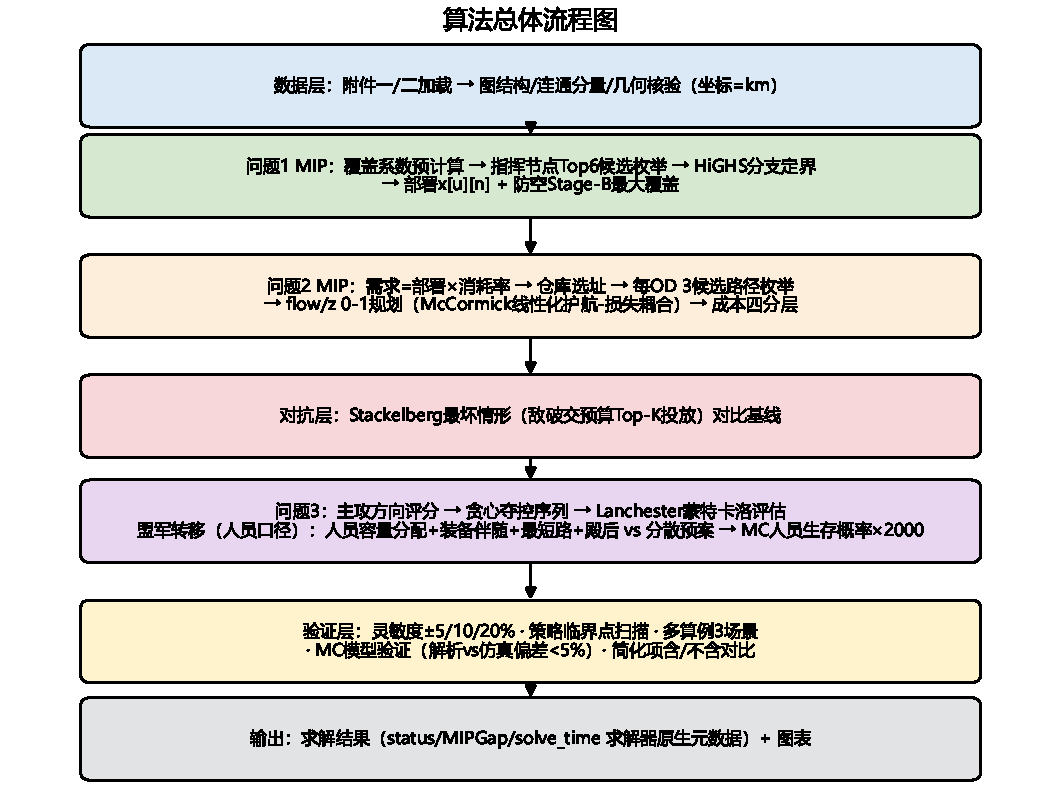
\includegraphics[width=0.62\textwidth]{result_bundle/figures/fig9_algorithm_flowchart.pdf}
\caption{算法总体流程图}
\label{fig:flowchart}
\end{figure}

图~\ref{fig:flowchart} 自顶向下展示了六个层次。数据层（蓝色）完成附件加载、图结构构建与坐标单位核验；问题一层（绿色）先预计算覆盖系数，再枚举指挥节点候选并以分支定界求解部署 MIP，防空配置作为第二阶段的最大覆盖问题解耦求解；问题二层（橙色）由部署量乘以消耗率生成需求，仓库选址后枚举每对起讫点的候选路径，用 0-1 规划与 McCormick 线性化求解；对抗层（红色）将敌方破交预算的最优响应对比基线；问题三层（紫色）分进攻与转移两条支线；验证层（黄色）汇总全部稳健性检验。各层输出统一汇入中间结果文件，其中求解状态、MIPGap 与求解时间均为求解器原生元数据透传，避免人工转述误差。

\subsection{双方兵力部署与指挥节点选址模型（问题一）}

\subsubsection{部署效能指标与 MIP 模型建立}

记己方节点集为 $\mathcal{O}_c$、敌方节点集为 $\mathcal{E}_c$。决策变量 $x_{u,n}\in\mathbb{Z}_+$ 表示单位类型 $u$ 在节点 $n$ 的部署数量。综合效能由火力覆盖、生存、指挥通信距离三项构成：
\begin{equation}
\max\ \varphi_c = w_1\frac{F_c}{F_{max}} + w_2\frac{S_c}{S_{max}} - w_3\frac{D_c}{D_{max}},\qquad (w_1,w_2,w_3)=(0.5,0.3,0.2)
\label{eq:phi}
\end{equation}

火力覆盖效能按目标价值加权求和。定义覆盖系数 $\mathrm{cov}_{u,n,m}=\mathbb{I}(\|p_n-p_m\|_2\le R_u)$，即单位 $u$ 在节点 $n$ 能否以射程 $R_u$ 覆盖敌节点 $m$；火炮射程取阵营最大射程（苏军 V3 为 16.8 km、盟军光棱火炮为 13.0 km），坦克取直射距离假设 A-02，动员兵与空中单位不计火力覆盖贡献。若同一敌节点 $m$ 被多支部队覆盖，简单求和会把重复覆盖计为多份战果，高估效能。为此引入有效覆盖数 $y_m=\min\{\sum_{u,n}\mathrm{cov}_{u,n,m}\,x_{u,n},\ 3\}$，即单目标有效覆盖次数上限为 3，超出的边际贡献计 0：
\begin{equation}
F_c=\sum_{m\in\mathcal{E}_c} v_m\,y_m,\qquad v_m=d_m,\qquad F_{max}=3\sum_{m\in\mathcal{E}_c}d_m
\label{eq:F}
\end{equation}
其中归一化常数 $F_{max}$ 取全部敌节点均被有效覆盖 3 次时的理论上限。$y_m$ 与部署量的耦合由线性约束 $y_m\le\sum_{u,n}\mathrm{cov}_{u,n,m}x_{u,n}$ 与上界 $y_m\le 3$ 刻画，最大化目标会自然将 $y_m$ 推到实际覆盖数与 3 的较小者，无需分段函数。

生存效能按节点防御强度与单位生存系数加权：
\begin{equation}
S_c=\sum_{u,n} d_n\,\mathrm{surv}_u\,x_{u,n},\qquad S_{max}=\sum_u N_{c,u}\,\mathrm{surv}_u
\label{eq:S}
\end{equation}
其中 $\mathrm{surv}_u$ 按装甲与隐蔽性估计：重型 0.85、中型 0.7、轻型 0.6、火炮 0.5、动员兵 0.4、空中 0.3。$S_{max}$ 为全部兵力集中于最高防御节点时的理论上界。防空加成效能 $S_{bonus}$ 在第二阶段计算（见第 5.2.3 小节），不进入部署 MIP 的目标。

指挥通信距离为部署量加权的路网平均距离。设候选指挥节点为 $z$，$\mathrm{dist}(n,z)$ 为 Dijkstra 路网最短路距离\cite{ref5}：
\begin{equation}
D_c=\frac{\sum_{u,n}x_{u,n}\,\mathrm{dist}(n,z)}{\sum_u N_{c,u}},\qquad D_{max}=43.335\ \mathrm{km}
\label{eq:D}
\end{equation}
$D_{max}$ 为主分量路网直径的采样估计（40 个随机源点的最短路最大值），用于把距离项归一到 $[0,1]$ 尺度。三项归一化后量纲统一为无量纲，加权求和才有意义；权重 $(0.5,0.3,0.2)$ 按题目语义排序（火力优先、生存次之、通信再次），并在第~\ref{sec:sens}~节做 $\pm20\%$ 扰动检验。

把式~\eqref{eq:F}--\eqref{eq:D} 代入式~\eqref{eq:phi}，目标对决策变量是线性的，$x_{u,n}$ 的目标系数为
\begin{equation}
\frac{w_2\,d_n\,\mathrm{surv}_u}{S_{max}}-\frac{w_3\,\mathrm{dist}(n,z)}{N_{total}\,D_{max}}
\label{eq:coef}
\end{equation}
$y_m$ 的系数为 $w_1 d_m/F_{max}$。约束条件如下：
\begin{align}
&\text{(C1 仅己方节点)} && x_{u,n}=0,\quad n\notin\mathcal{O}_c \label{eq:c1}\\
&\text{(C2 兵力守恒)} && \sum_{n}x_{u,n}=N_{c,u},\quad u\ne\text{空中} \label{eq:c2}\\
&\text{(C4 空中上限)} && \sum_{n}x_{\text{空中},n}\le \alpha\,N_{c,\text{空中}},\quad \alpha=10\% \label{eq:c4}\\
&\text{(C5 咽喉覆盖)} && \sum_{u,n:(n,m_e)\in\mathrm{cov}_u}x_{u,n}\ge 1,\quad \forall\ \text{咽喉边敌方端点}\ m_e \label{eq:c5}\\
&\text{(P2 节点容量)} && 0\le x_{u,n}\le \lfloor 0.15\,N_{c,u}\rfloor \label{eq:c9}
\end{align}
约束 C2 对地面五类单位取等式，即全部地面兵力必须部署；空中单位按题目“不宜部署过多”取上限不等式（A-04），其余留作预备队。C5 要求每条跨阵营边的敌方端点至少被 1 个火力单位覆盖，保证咽喉处于火力封锁之下。P2 将单节点部署限制在该类型总量的 15\% 以内，防止解退化为把所有兵力堆在个别高防御节点。防空炮阵地独立于兵力体系（不占用 C2 的兵力守恒），在第二阶段单独选址。

\subsubsection{指挥节点候选生成与求解算法选择}

指挥节点须兼顾通信、隐蔽与抗毁三方面。先以多准则评分从己方主分量节点中选出 6 个候选：以防御强度加权的己方部署重心 $(\bar x,\bar y)$ 为参考，
\begin{multline}
\mathrm{score}(n)=0.4\Big(1-\frac{\|p_n-(\bar x,\bar y)\|_2}{\max_{n'}\|p_{n'}-(\bar x,\bar y)\|_2}\Big)\\
+0.3\Big(1-0.5\,d_n-0.5\,\frac{\min(\deg(n),6)}{6}\Big)+0.3\,d_n
\label{eq:cmdscore}
\end{multline}
三项分别对应靠近重心的通信便利、低防御暴露与低度数的隐蔽性、防御强度代表的抗毁能力。对每个候选 $z$ 重新计算 $\mathrm{dist}(n,z)$ 并求解一次部署 MIP，取 $\varphi$ 最大的候选为主选指挥节点，其余候选按评分取 3 个备选。候选数取 6 是求解时间与覆盖度的折中：每候选求解约 0.2--0.4 s，6 候选总耗时在 3 s 以内。

求解算法对比三种候选\cite{ref2}。其一，分支定界法（pulp 调用 CBC/HiGHS 求解器）：模型经式~\eqref{eq:coef} 线性化后为纯线性 MIP，分支定界能给出全局最优证明，本规模（苏军约 1600、盟军约 1000 个整数变量）下秒级求解。其二，贪心启发式：按节点边际贡献逐个放置兵力，实现简单但无最优性保证，且覆盖耦合下局部最优与全局差距不可控。其三，连续松弛加取整：求解快但取整后可能违反兵力守恒与咽喉覆盖约束，修复取整解的代价不低于直接求解原问题。选择分支定界法，理由是模型结构允许精确求解且规模在开源求解器能力之内，贪心与松弛取整仅在求解器超时的情形下作为后备。

\subsubsection{防空配置的两阶段解耦}

防空炮阵地选址在部署确定后进行（Stage B）：10 个据点覆盖已部署兵力，最大化覆盖权重和。设部署节点 $n$ 的权重为 $q_n=\sum_u \mathrm{surv}_u\,x_{u,n}$，决策变量 $a_p\in\{0,1\}$ 表示节点 $p$ 是否设防空据点，$c_n\in[0,1]$ 表示部署节点 $n$ 是否被覆盖：
\begin{equation}
\max\ \sum_n q_n c_n,\qquad \text{s.t.}\ \ \sum_p a_p=10,\quad c_n\le\sum_{p:\|p_n-p_p\|_2\le R_{aa}}a_p
\label{eq:aa}
\end{equation}
\begin{sloppypar}
覆盖内部署单位的生存率提升 20\%，对应加成 $S_{bonus}=0.2\sum_{n\in\text{覆盖}}d_n\sum_u\mathrm{surv}_u x_{u,n}$。两阶段解耦的合理性在于：防空据点不占用兵力守恒约束，且生存加成只改变效能值、不改变部署 MIP 的可行域；联合求解虽理论更优，但会把模型规模扩大一倍以上，而第~\ref{sec:sens}~节的扫描表明防空布局对半径参数高度稳健，解耦的次优代价可忽略。
\end{sloppypar}

\subsubsection{求解结果与最优性验证}

双方 MIP 均由分支定界法证明全局最优：苏军 status=optimal、MIPGap=0、求解时间 0.225 s；盟军 status=optimal、MIPGap=0、求解时间 0.138 s。MIPGap 为 0 意味着求解器已证明不存在更优整数解，这是精确算法相对启发式的本质优势。结果汇总见表~\ref{tab:q1res}。

\begin{table}[H]
\centering
\caption{问题一求解结果汇总}
\label{tab:q1res}
\zihao{5}
\begin{tabular}{lccccccc}
\toprule
阵营 & $\varphi$ & $F$ & $S_{base}$ & $S_{bonus}$ & $D$/km & 指挥节点 & 部署节点数 \\
\midrule
苏军 & 0.7688 & 276.24 & 4017.37 & 803.47 & 2.279 & 136 & 10 \\
盟军 & 0.7732 & 411.09 & 7796.90 & 1559.38 & 1.872 & 384 & 10 \\
\bottomrule
\end{tabular}
\end{table}

苏军主选指挥节点为 136，备选 187、137、358；盟军主选 384，备选 411、255、214。一个值得注意的现象是：盟军多准则评分第一的节点是 411（评分 0.7665），而 384 的评分仅列第三（0.7475），但逐候选重解 MIP 后 384 的综合效能 $\varphi=0.7732$ 最高。评分只反映指挥节点自身的通信、隐蔽、抗毁属性，$\varphi$ 还包含该节点作为指挥中枢时全部署的通信距离成本，两者的排序差异说明指挥节点选址必须与部署方案耦合评估，单靠多准则评分预排序会选错。

部署方案呈现“前沿多点集中”结构，双方均使用 10 个部署节点，见表~\ref{tab:q1deploy}。苏军火炮（V3）依托 16.8 km 射程在纵深节点 136、142、344、358、386、413、137 各部署 1050 门，坦克与动员兵前推至 28、86 等靠近咽喉的节点；盟军火炮数量是苏军的两倍（14000 对 7000），在 134、140、150、247、255、384 各部署 2100 门，但光棱火炮射程只有 13.0 km，必须更靠前部署才能覆盖目标。空中单位按上限约束少量集中部署（苏军 50 架于 386、盟军 30 架于 384），符合题目“不宜部署过多”的定性要求。

\begin{table}[H]
\centering
\caption{问题一双方主要部署节点与数量（节选）}
\label{tab:q1deploy}
\zihao{5}
{\setlength{\tabcolsep}{5pt}
\begin{tabular}{llrrrrrr}
\toprule
阵营 & 节点 & 动员兵(万人) & 轻型(辆) & 中型(辆) & 重型(辆) & 火炮(门) & 空中(架) \\
\midrule
苏军 & 136 & 18 & -- & -- & -- & 1050 & -- \\
苏军 & 28 & -- & 63 & 45 & 27 & -- & -- \\
苏军 & 386 & 18 & 63 & 45 & 27 & 1050 & 50 \\
苏军 & 86 & -- & -- & 30 & 18 & 3 & -- \\
盟军 & 384 & 15 & 120 & 85 & 51 & 2100 & 30 \\
盟军 & 134 & 15 & 120 & 85 & 51 & 2100 & -- \\
盟军 & 218 & 10 & 80 & 60 & 34 & 1391 & -- \\
盟军 & 255 & 15 & 120 & 85 & 51 & 2100 & -- \\
\bottomrule
\end{tabular}}
\end{table}

图~\ref{fig:deploy} 展示了双方部署的空间分布。黑色圆圈大小表示节点部署总量，金色五角星为主选指挥节点，浅黄五角星为备选，绿色三角为防空据点。苏军部署沿南侧前线与纵深火炮阵地两层展开，指挥节点 136 位于前线群中央；盟军部署更贴近前线，指挥节点 384 与各部署节点的距离普遍更短（$D=1.872$ km 对苏军 2.279 km）。两军的防空据点均与部署节点重合或紧邻，这是 Stage B 最大覆盖模型的直接结果。

\begin{figure}[H]
\centering
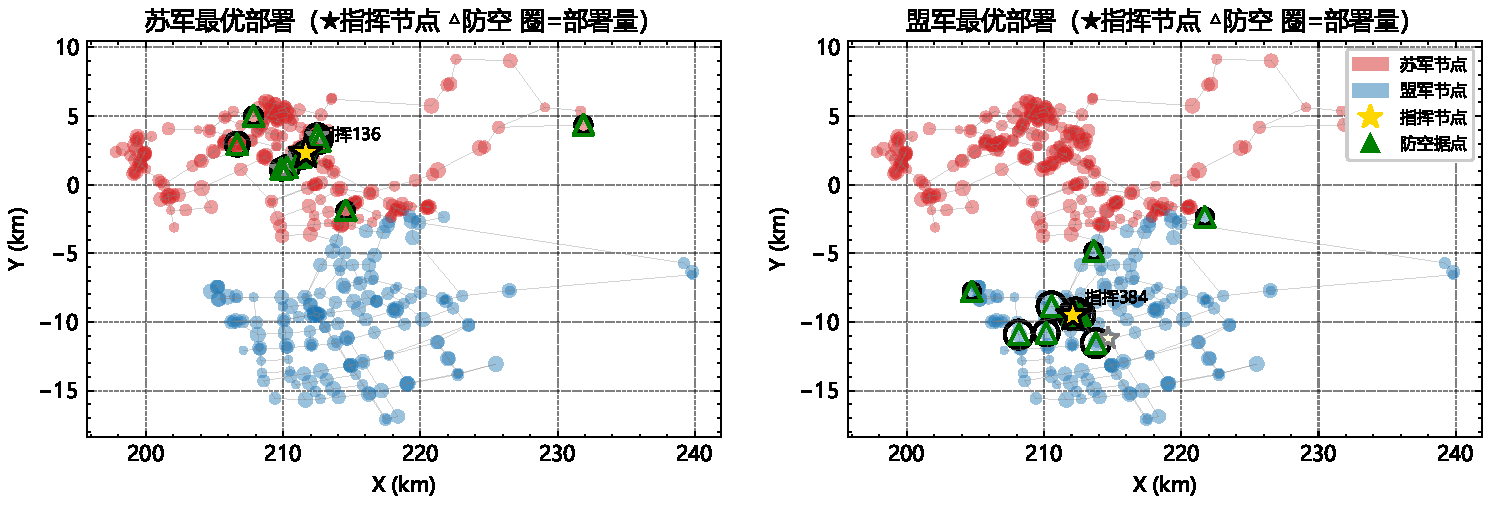
\includegraphics[width=0.80\textwidth]{result_bundle/figures/fig1_deployment_map.pdf}
\caption{问题一双方最优部署分布（左：苏军，右：盟军；圆圈大小表示部署总量，★指挥节点，△防空据点）}
\label{fig:deploy}
\end{figure}

图~\ref{fig:deploycomp} 以堆叠柱状图对比双方部署构成。盟军各型装备的部署数量整体高于苏军（火炮 14000 对 7000、轻型 800 对 420），空中单位受上限约束分别只部署 30 与 50 架。动员兵按万人粒度部署，苏军 125 个单位、盟军 100 个单位全部落位。该图直观呈现了双方的兵力禀赋差异：盟军数量占优、苏军坦克质量占优（重型 180 辆天启对盟军 340 辆光棱中重型合计，苏军单车火力系数更高），这一非对称性为问题三的进攻想定提供了背景。

\begin{figure}[H]
\centering
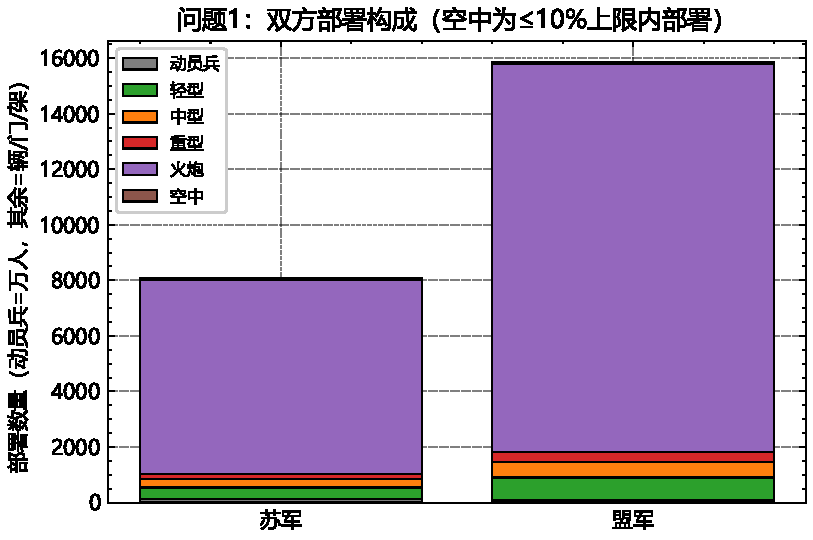
\includegraphics[width=0.46\textwidth]{result_bundle/figures/fig2_deployment_composition.pdf}
\caption{问题一双方部署构成（空中为不超过 10\% 上限下的部署量）}
\label{fig:deploycomp}
\end{figure}

\subsubsection{结果验证与量级合理性}

问题一为确定性 MIP，无随机参数，蒙特卡洛模型验证不适用；其验证维度为最优性证明（MIPGap=0）与参数稳健性扫描（第~\ref{sec:sens}~节），两者相互独立。活跃约束方面，六类兵力守恒约束全部紧（slack 为 0，即各类型部署合计恰等于兵力总量），全部咽喉覆盖约束紧（每条咽喉被不少于 1 个火力单位覆盖），说明兵力没有冗余、咽喉封锁没有富余，解处在资源充分利用的边界上。

结果量级合理性核查如下。部署节点数 10 个，占己方主分量节点（苏军约 245、盟军约 168）的 4\%--6\%，符合“要点防御”的军事常识；指挥通信距离 2.279 km 与 1.872 km 远小于战场直径 43.3 km，指挥半径合理；综合效能 0.7688 与 0.7732 介于 0 与 1 之间且双方接近，反映非对称兵力下攻防大体均衡，与题目“形成相对稳定的战场动态平衡”的设定一致。

\subsection{三类补给分配与供应优化模型（问题二）}

\subsubsection{需求生成与仓库选址}

补给需求由问题一部署派生。对部署节点 $n$，记装备数量为 $E_n$（辆/门，不含动员兵）、动员兵为 $I_n$（万人），物资 $k\in\{$弹药，燃油，维修包$\}$ 的日需求为
\begin{equation}
\mathrm{Demand}_{c,k,n}=\rho^{eq}_k\,\frac{E_n}{100}+\rho^{inf}_k\,I_n
\label{eq:demand}
\end{equation}
其中消耗率（假设 3）为 $\rho^{eq}=(0.8,0.6,0.2)$ 吨/百辆、$\rho^{inf}=(0.3,0.15,0.05)$ 吨/万人，动员兵三类合计 0.5 吨/万人。苏军总需求 189.7 吨/日，盟军 301.84 吨/日。仓库选址取己方主分量内纵深与防御兼优的 3 个节点：苏军纵深向北（纵坐标大），盟军纵深向南（纵坐标小），评分 $0.6\times$ 纵深归一值 $+0.4\times$ 防御强度。求得苏军仓库为 275、119、41，盟军为 296、318、352。

\subsubsection{成本四分层与补给网络模型}

后勤总成本分解为四类独立分项，各有独立符号、公式与经济含义：
\begin{align}
C_{trans}&=\sum_r \mathrm{trips}_r\,L_r\,c_{km}, && c_{km}=20\ \text{元/km$\cdot$车} \label{eq:ctrans}\\
C_{escort}&=\sum_r e_r\,\mathrm{trips}_r\,c_{esc}, && c_{esc}=500\ \text{元/车次} \label{eq:cescort}\\
C_{loss}&=\sum_r \mathrm{flow}_r\,P_{int,r}\,(1-0.5\,e_r)\,c_{unit}, && c_{unit}=1000\ \text{元/吨} \label{eq:closs}\\
C_{labor}&=W\times c_w, && c_w=300\ \text{元/人$\cdot$日} \label{eq:clabor}
\end{align}
式~\eqref{eq:ctrans} 为车队运行的直接里程成本，与路径长度、发车频次成正比；式~\eqref{eq:cescort} 为武装护航的资源消耗，仅在启用护航的路径发生；式~\eqref{eq:closs} 为敌方破交的期望物资损失，是对手行动的期望代价，护航以 50\% 的削减率降低该项；式~\eqref{eq:clabor} 为后勤工人（司机加装卸）的维持成本。总成本为四项之和：
\begin{equation}
\mathrm{TC}=C_{trans}+C_{escort}+C_{loss}+C_{labor}
\label{eq:tc}
\end{equation}

路径拦截概率由边风险复合而来。设路径 $p=(n_0,n_1,\dots,n_K)$ 经过的边序列为 $e_1,\dots,e_K$，各边独立拦截：
\begin{equation}
P_{int}(p)=1-\prod_{i=1}^{K}(1-\mathrm{risk}_{e_i})
\label{eq:pathrisk}
\end{equation}
该式从“全程安全等于各边均安全”的独立性假设直接推出。决策变量为路径流量 $\mathrm{flow}_r\ge 0$（吨/日，连续）与护航决策 $e_r\in\{0,1\}$。路径集预枚举：对每个“仓库—需求节点”对，用最短路与边禁用扰动法生成 3 条候选路径（最短路、次短路、风险加权最短路，思路源于 Yen 的 k 短路枚举\cite{ref6}），按 $L(1+3P_{int})$ 混合排序保留前 3。约束包括需求满足 $\sum_{r\to n}\mathrm{flow}_r\ge\mathrm{Demand}_n$、每节点启用护航的路径不超过 2 条（防止过度分散），以及护航—损失耦合的线性化约束（下述）。

护航项 $e_r\cdot\mathrm{flow}_r$ 是双线性项，引入辅助变量 $w_r=e_r\,\mathrm{flow}_r$ 并以 McCormick 凸包线性化。设流量上界 $M_n=3\,\mathrm{Demand}_n$：
\begin{equation}
w_r\le M_n e_r,\quad w_r\le \mathrm{flow}_r,\quad w_r\ge \mathrm{flow}_r-M_n(1-e_r),\quad w_r\ge 0
\label{eq:mccormick}
\end{equation}
由于 $e_r\in\{0,1\}$，式~\eqref{eq:mccormick} 在整数解处精确成立（$e_r=1$ 时 $w_r=\mathrm{flow}_r$，$e_r=0$ 时 $w_r=0$），不引入近似。目标中损失项写为 $\mathrm{risk}_r\,c_{unit}(\mathrm{flow}_r-0.5\,w_r)$，即护航削减一半期望损失。

需要说明计算口径：MIP 内部对护航成本采用固定份额线性化近似（$e_r$ 的系数按需求均分份额的车次数计算），因此 MIP 目标值（苏军 81690.4、盟军 107511.6 元/日）低于真实成本。求解完成后，对 MIP 给出的路径、流量与护航组合按式~\eqref{eq:ctrans}--\eqref{eq:clabor} 逐项重算，得到真实总成本 TC。本文一律以重算值为准，差距的量化见第~\ref{sec:err}~节。

\subsubsection{破交—护航对抗的 Stackelberg 刻画}

敌方破交策略与我方护航决策构成序贯对抗：我方（领导者）先承诺路径、流量与护航组合，敌方（追随者）观察后将有限破交预算投向期望截获收益最大的路径。敌方的最优响应为按“流量$\times$货值/护航强度”排序，将预算（5 条路径）投向排名前五的路径，集中打击使这些路径的有效损失上升。最坏情形总成本为
\begin{equation}
\mathrm{TC}_{worst}=\mathrm{TC}+\sum_{r\in\mathcal{H}}\mathrm{flow}_r\,\mathrm{risk}_r\,c_{unit}\times 0.5
\label{eq:worst}
\end{equation}
其中 $\mathcal{H}$ 为敌方选中的 Top-5 路径集合。

均衡论证按零和博弈的纳什均衡（鞍点）标准给出。其一，单方偏离收益比较：我方在敌方打击集合 $\mathcal{H}$ 固定时偏离当前护航组合，等于放弃 MIP 最优解，总成本不会下降（MIPGap=0 已证明全局最优，任何可行偏离的目标值不小于最优值）；敌方在我方方案固定时偏离 Top-5 打击集合，等于放弃按收益排序的最优响应，截获损失不会增加。双方均无单方偏离动机。其二，帕累托区分：零和博弈中帕累托概念退化为 minimax 值，纳什均衡即鞍点，不存在帕累托改进空间，此处显式标注。表~\ref{tab:game} 汇总了偏离分析。

\begin{table}[H]
\centering
\caption{破交—护航对抗的单方偏离收益比较（零和，苏军口径）}
\label{tab:game}
\zihao{5}
\begin{tabular}{p{2.2cm}p{5.8cm}p{5.2cm}}
\toprule
参与方 & 策略状态 & 单方偏离的后果 \\
\midrule
我方（领导者） & 当前护航组合（MIP 最优，$\mathrm{TC}=109614$ 元/日） & 偏离后成本不降（MIPGap=0，全局最优） \\
敌方（追随者） & Top-5 打击集合（额外损失 55721 元/日） & 偏离后截获损失不增（排序最优响应） \\
\bottomrule
\end{tabular}
\end{table}

\subsubsection{求解结果、模型验证与结果分析}

双方 MIP 均证明全局最优（status=optimal，MIPGap=0，求解时间 0.391 s 与 0.07 s）。最优补给方案：苏军启用 10 条配送路径，盟军 10 条，全部路径启用护航。表~\ref{tab:q2routes} 给出方案明细（路径以仓库与需求节点标识）。

\begin{table}[H]
\centering
\caption{问题二最优补给方案（流量降序，全部路径护航，每车装载 10 吨）}
\label{tab:q2routes}
\zihao{5}
\resizebox{\textwidth}{!}{
\begin{tabular}{llrrrrr}
\toprule
阵营 & 仓库$\to$需求节点 & 路径长/km & 拦截风险 & 流量/(吨/日) & 车次/(次/日) & 发车周期/h \\
\midrule
苏军 & 119$\to$386 & 7.518 & 0.7362 & 28.76 & 2.88 & 8.34 \\
苏军 & 119$\to$142 & 5.489 & 0.6902 & 27.96 & 2.80 & 8.58 \\
苏军 & 119$\to$344 & 8.725 & 0.8426 & 27.96 & 2.80 & 8.58 \\
苏军 & 119$\to$358 & 9.551 & 0.8567 & 27.96 & 2.80 & 8.58 \\
苏军 & 119$\to$413 & 9.753 & 0.8390 & 27.96 & 2.80 & 8.58 \\
苏军 & 119$\to$136 & 8.030 & 0.8346 & 25.80 & 2.58 & 9.30 \\
苏军 & 119$\to$137 & 8.449 & 0.8191 & 20.28 & 2.03 & 11.84 \\
苏军 & 119$\to$28 & 1.568 & 0.2464 & 2.16 & 0.22 & 111.11 \\
苏军 & 119$\to$86 & 15.448 & 0.9012 & 0.82 & 0.08 & 294.12 \\
苏军 & 275$\to$283 & 7.885 & 0.2464 & 0.05 & 0.00 & 5000.00 \\
盟军 & 318$\to$384 & 7.171 & 0.6742 & 45.68 & 4.57 & 5.25 \\
盟军 & 318$\to$134 & 4.449 & 0.4416 & 45.20 & 4.52 & 5.31 \\
盟军 & 318$\to$140 & 10.732 & 0.6652 & 45.20 & 4.52 & 5.31 \\
盟军 & 318$\to$150 & 9.131 & 0.7361 & 45.20 & 4.52 & 5.31 \\
盟军 & 318$\to$247 & 6.935 & 0.6327 & 45.20 & 4.52 & 5.31 \\
盟军 & 318$\to$255 & 7.256 & 0.7599 & 45.20 & 4.52 & 5.31 \\
盟军 & 318$\to$218 & 8.723 & 0.6152 & 30.04 & 3.00 & 7.99 \\
盟军 & 318$\to$77 & 12.566 & 0.8301 & 0.05 & 0.00 & 5000.00 \\
盟军 & 318$\to$166 & 22.756 & 0.9807 & 0.05 & 0.00 & 5000.00 \\
盟军 & 318$\to$380 & 15.574 & 0.8990 & 0.05 & 0.00 & 5000.00 \\
\bottomrule
\end{tabular}
}
\end{table}

表~\ref{tab:q2routes} 中，主力路径的拦截风险集中在 0.6--0.9 区间，因为这些路径必须穿越或贴近前线咽喉区域；小流量路径（边缘哨所补给）风险虽高但损失期望小，发车周期长达数千小时，属低频补给。成本构成见表~\ref{tab:q2cost}。

\begin{table}[H]
\centering
\caption{问题二成本四分层与总成本（元/日）}
\label{tab:q2cost}
\zihao{5}
\begin{tabular}{lrrrrrr}
\toprule
阵营 & $C_{trans}$ & $C_{escort}$ & $C_{loss}$ & $C_{labor}$ & TC（合计） & MIP 内部目标值 \\
\midrule
苏军 & 3096.5 & 9485.0 & 75432.2 & 21600.0 & 109613.7 & 81690.4 \\
盟军 & 4664.4 & 15092.0 & 97816.6 & 28200.0 & 145773.0 & 107511.6 \\
\bottomrule
\end{tabular}
\end{table}

成本结构中破交损失占绝对主导：苏军 $C_{loss}$ 占 TC 的 68.8\%，盟军占 67.1\%；护航成本只占 8.7\% 与 10.4\%，却把主力路径的损失期望削减一半，是典型的“小投入换大损失规避”。人力成本占 19.7\% 与 19.3\%，运输成本占比最低（2.8\% 与 3.2\%）。

盟军火炮数量是苏军的两倍（14000 对 7000），后勤总成本反而高出 33.0\%（145773 对 109614 元/日）。根因在于射程与部署位置的联动：光棱火炮 13.0 km 的射程短于 V3 的 16.8 km，盟军火炮必须靠前部署才能覆盖目标，部署节点贴近前线使补给路径长且暴露（盟军最长主力路径 10.732 km，苏军 9.753 km）。

虽然盟军主力路径的平均拦截风险（0.6464）低于苏军（0.8026），但盟军单路径流量约为苏军的 1.6 倍（45.2 吨/日对 27.96 吨/日），损失期望 $C_{loss}=\sum \mathrm{flow}_r P_{int,r} c_{unit}$ 由流量主导，最终盟军 $C_{loss}$ 达 97816.6 元/日，高于苏军的 75432.2。数量优势没有转化为后勤优势，这是本题一个反直觉的发现；交叉验证依据是两组结果来自同一模型同一代码、仅输入兵力与装备参数不同，差异只能由部署位置、路径结构与流量规模解释。

图~\ref{fig:routes} 展示了双方补给网络的空间形态。实线为护航路径（全部路径均护航，故图中均为实线），线宽与流量成正比，金色方块为仓库。苏军仓库 119 承担了 9 条路径中的 9 条，呈单枢纽辐射状；盟军仓库 318 同样承担主力。路径在穿越前线区域时明显绕行，以长度换风险，体现了式~\eqref{eq:tc} 中运输成本与损失成本的权衡。

\begin{figure}[H]
\centering
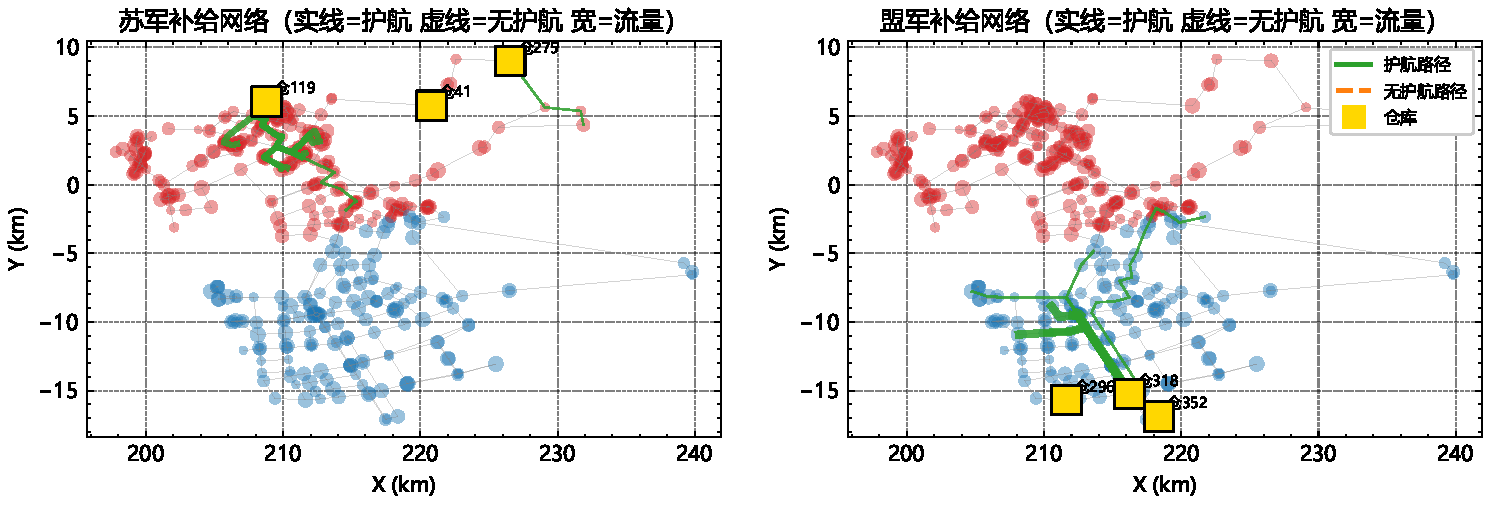
\includegraphics[width=0.80\textwidth]{result_bundle/figures/fig3_supply_routes.pdf}
\caption{问题二双方最优补给网络（线宽表示流量，金色方块为仓库）}
\label{fig:routes}
\end{figure}

图~\ref{fig:cost} 以分组柱状图对比双方四类成本。破交损失柱显著高于其余三类，护航柱约为损失柱的八分之一，直观支持“护航是必需投入”的判断。两军成本谱的形状相似（损失主导、人力次之），盟军整体高出约三分之一，与表~\ref{tab:q2cost} 一致。

\begin{figure}[H]
\centering
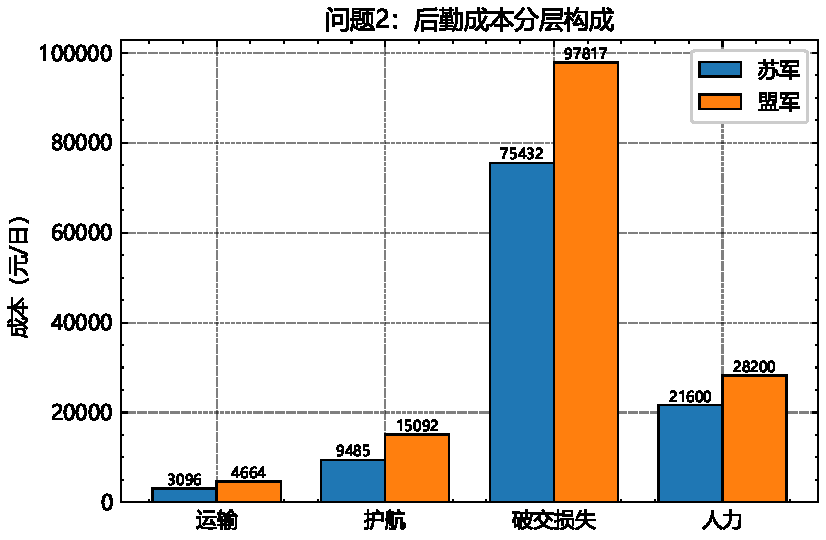
\includegraphics[width=0.46\textwidth]{result_bundle/figures/fig4_cost_decomposition.pdf}
\caption{问题二后勤成本四分层构成（元/日）}
\label{fig:cost}
\end{figure}

\textbf{模型验证（蒙特卡洛）}。问题二含破交随机性，用伯努利拦截仿真交叉验证解析期望损失：对每条路径按拦截概率 $P_{int,r}(1-0.5e_r)$ 独立抽样，命中则损失该路径全部流量货值，重复 2000 次。结果：苏军解析值 75432.2 元/日，仿真均值 74890.9，偏差 0.72\%；盟军解析值 97816.6，仿真均值 96310.9，偏差 1.54\%（解析值与表~\ref{tab:q2cost} 的 $C_{loss}$ 为同一量的统一舍入表述）。两处偏差均小于 5\%，模型验证通过。损失为低频高额的复合分布（std/mean 达 46.70\%/54.61\%），2000 次下均值偏差已达标；重尾分布下将仿真次数增至 $10^4$ 以进一步压缩标准误，列为后续工作。

需要说明收敛口径：仿真损失的标准差与均值之比为 46.70\%（苏军）与 54.61\%（盟军），按 std/mean 阈值判定为“not converged”，但这源于损失是低频高额事件（复合分布的内在离散），并非均值估计未收敛；均值偏差（0.72\%/1.54\%）才是模型验证的判据，两个口径在此一并披露。

\textbf{消耗模式}。完全不补给时，按独立公式计算维持前线所需投入：苏军需后勤工人 61 人、运输车辆 10 辆（总需求 189.7 吨/日，平均单程 2.14 h，日周转 11.24 次）；盟军需工人 91 人、车辆 10 辆（总需求 301.84 吨/日）。补给模式下实际用工为苏军 72 人、盟军 94 人（含装卸），车辆 16 与 12 辆。

\textbf{Stackelberg 最坏情形}。敌方将破交预算投向流量最大的 5 条路径（苏军路径 16、7、10、13、18，盟军路径 18、0、3、6、12），苏军额外损失 55721.0 元/日，$\mathrm{TC}_{worst}=165334.7$，较基线上升 50.83\%；盟军额外损失 71341.0，$\mathrm{TC}_{worst}=217114.0$，上升 48.94\%。对照口径为含人力 $\mathrm{TC}_{total}$（与式~\eqref{eq:tc} 的 objective 口径一致）：破交追加损失只作用于货物损失项，人力成本在对抗情形下不变，故 $\mathrm{TC}_{worst}=\mathrm{TC}_{total}+\text{extra\_loss}$\footnote{若以不含人力成本口径（苏军基线 88013.7、盟军 117573.0 元/日）为参照，同一额外损失对应增幅 $+63.31\%$ 与 $+60.68\%$；本文一律以含人力 $\mathrm{TC}_{total}$ 为主口径。}。这组数字把假设 A-01 的不确定性折算为明确的鲁棒性成本：静态风险基线下的方案在对抗最坏情形下成本上浮约五成，决策者应以此为预算上限做准备。

图~\ref{fig:stackelberg} 将两军基线成本与对抗最坏情形成本并排对比，苏军绝对增量 55721.0 元/日、盟军 71341.0 元/日，盟军因流量更大、单路径损失期望更高，对抗代价的绝对值更大，但相对增幅（48.94\%）反而低于苏军（50.83\%），说明苏军补给网络对集中打击的相对脆弱性更高。

\begin{figure}[H]
\centering
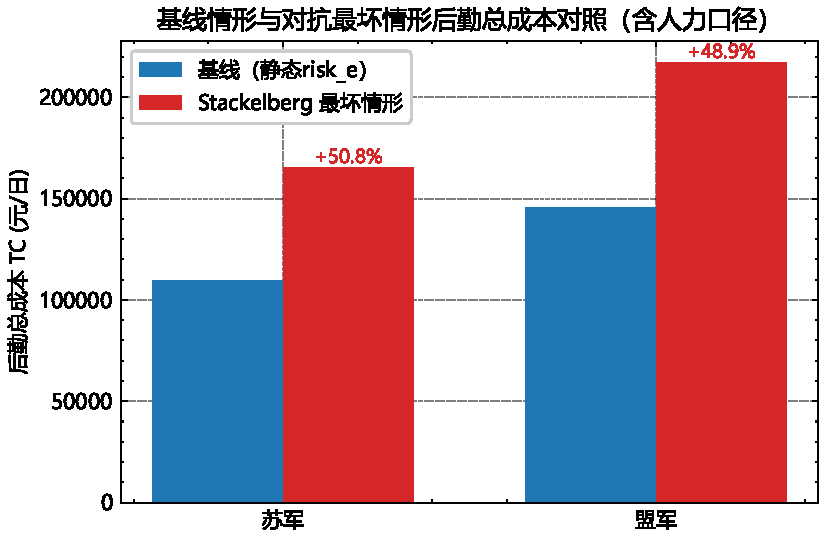
\includegraphics[width=0.46\textwidth]{result_bundle/figures/fig13_q2_a01_baseline_vs_stackelberg.pdf}
\caption{A-01 破交概率的基线情形与 Stackelberg 对抗最坏情形总成本对照（元/日，含人力）}
\label{fig:stackelberg}
\end{figure}

\subsection{苏军进攻方案与盟军战略转移模型（问题三）}

\subsubsection{主攻方向评分与夺控序列构造}

主攻方向在 8 条跨阵营边中选择。对苏军端 $a_s$、盟军端 $a_m$ 的边，评分综合敌方防御弱点、走廊价值与纵深方向：
\begin{equation}
\mathrm{score}=0.5\,(1-d_{a_m})+0.3\,\frac{\min(\deg(a_m),6)}{6}+0.2\,\frac{1}{1+|Y_{a_s}-Y_{a_m}|}
\label{eq:axis}
\end{equation}
第一项偏好防御薄弱的突破口，第二项偏好端点度数高的走廊（攻入后机动选择多），第三项偏好纵向落差小的边（推进方向顺畅）。评分排序见表~\ref{tab:axes}。

\begin{table}[H]
\centering
\caption{问题三苏军主攻方向候选评分（前 4 名）}
\label{tab:axes}
\zihao{5}
\begin{tabular}{lrrr}
\toprule
进攻边 & 边长/km & 敌方端点防御 & 评分 \\
\midrule
55$\to$372 & 0.567 & 0.58 & 0.5133 \\
251$\to$166 & 1.289 & 0.45 & 0.4906 \\
39$\to$229 & 1.101 & 0.67 & 0.4556 \\
366$\to$74 & 0.334 & 0.60 & 0.4537 \\
\bottomrule
\end{tabular}
\end{table}

主攻方向定为 55$\to$372：边长仅 0.567 km，走廊价值与纵深得分弥补了防御 0.58 的中等水平。需要指出，第一名与第二名（251$\to$166）的评分差仅 0.0227，次优边的防御更弱（0.45 对 0.58）但边长与走廊得分不利，翻转条件在第~\ref{sec:flip}~节专门讨论。

夺控序列从主攻边的盟军端点 372 出发贪心扩展：每步在当前节点的未访问盟军邻居中选取评分 $0.6(1-d_v)+0.4\,d_v$ 最大者（偏好低防御、兼顾战略价值），共 6 步，序列为
\begin{equation}
372\to 328\to 286\to 256\to 422\to 33\to 198
\label{eq:seq}
\end{equation}
第一梯队编成为重型 40\%、中型 30\%、动员兵 20\%、火炮 10\%，投入兵力为动员兵 125 万人、轻型 420 辆、中型 300 辆、重型 180 辆、火炮 7000 门、空中 50 架（取问题一主分量部署聚合值）。

每步战斗用 Lanchester 平方律蒙特卡洛评估\cite{ref8,ref12}。平方律刻画 aimed fire：双方损耗率与对方火力总量成正比，防御强度以 $(1+0.5d)$ 乘性修正。离散化数值格式为：每步长 $\Delta t=0.5$，火力总量 $\mathrm{fire}_a=\sum_u\lambda_u a_u$，损耗按总量比例摊到各单位：
\begin{equation}
a_u\leftarrow a_u\Big(1-\frac{\mathrm{fire}_d\,\Delta t\times 0.01}{\sum_{u'}a_{u'}}\Big),\qquad d_u\leftarrow d_u\Big(1-\frac{\mathrm{fire}_a\,\Delta t\times 0.01}{\sum_{u'}d_{u'}}\Big)
\label{eq:lanchester}
\end{equation}
初始兵力叠加乘性噪声（正态 $\sigma=0.15$，截断于 $[0.5,1.5]$ 倍），每步 500 次仿真、种子 2026 固定可复现。守军强度按 $k_{def}=0.5+0.3\,d$ 标定：守军总量为攻方单步投入的 $k_{def}$ 倍，兵种构成为动员兵 45\%、中型 25\%、重型 18\%、火炮 12\%。评估结果见表~\ref{tab:capture}。

\begin{table}[H]
\centering
\caption{问题三夺控序列各步战斗评估（每步 500 次蒙特卡洛，种子 2026）}
\label{tab:capture}
\zihao{5}
\begin{tabular}{lrrr}
\toprule
夺控节点 & 防御强度 & 攻方胜率 & 攻方剩余兵力比 \\
\midrule
328 & 0.08 & 1.000 & 0.9121 \\
286 & 0.89 & 0.982 & 0.8451 \\
256 & 0.41 & 1.000 & 0.8848 \\
422 & 0.65 & 0.994 & 0.8649 \\
33 & 0.19 & 1.000 & 0.9030 \\
198 & 0.14 & 1.000 & 0.9071 \\
\bottomrule
\end{tabular}
\end{table}

六步胜率均不低于 0.982，攻方剩余兵力比介于 0.8451 与 0.9121 之间，序列平均剩余比 0.8862。消耗最重的一步是节点 286（防御 0.89，全场最高），胜率降至 0.982、剩余比降至 0.8451，说明高防御节点即使兵力占优也要付出约 15\% 的消耗。序列整体可行（每步均为前一节点的邻接盟军节点，可行性约束紧），但胜率对标定系数 $k_{def}$ 敏感，局限见第~\ref{sec:err}~节。

\textbf{算法选择理由}。进攻序列本质是多阶段组合优化，对比三种算法：动态规划的状态为（已控节点集合，剩余兵力向量），状态空间 $O(2^n\times$ 兵力离散格$)$，$n=436$ 时不可行，即使限制在约 30 个走廊候选节点上，兵力连续维度仍使状态格爆炸；MIP 时序展开引入变量 $x_{n,t}\in\{0,1\}$（436 节点 $\times$ 10 阶段共 4360 个），但战斗损耗是双方兵力乘积项，大 M 线性化导致松弛极弱，分支定界难以收敛；贪心加 Lanchester 仿真的复杂度为 $O(k\cdot n\cdot MC)$（$k$ 为夺占步数），可行且每步有蒙特卡洛质量评估。

故采用贪心构造，并以“启发式、无全局最优保证”显式声明其最优性状态。建模阶段曾拟以走廊子图小规模 MIP 对照验证贪心解质量，因时序展开松弛过弱（如上分析）难以给出可靠的最优性差距参照值，该对照未实施，贪心解质量改以蒙特卡洛统计评估：确定性构造加固定种子保证可复现，步内方差由每步 500 次仿真吸收，跨步剩余比 std/mean 为 2.74\%，低于 5\% 阈值，判定收敛。

图~\ref{fig:attack} 展示了主攻方向与夺控序列的空间走向。红色粗箭头为主攻边 55$\to$372，暗红色虚线箭头依次连接 7 个夺控节点（编号 1--7）。序列自北向南楔入盟军防线，先取低防御节点 328 建立桥头堡，再向西、向南滚动扩展，避开防御 0.89 的节点 286 直至第 2 步才以优势兵力强攻，体现了贪心评分“先易后难、兼顾价值”的取舍。

\begin{figure}[H]
\centering
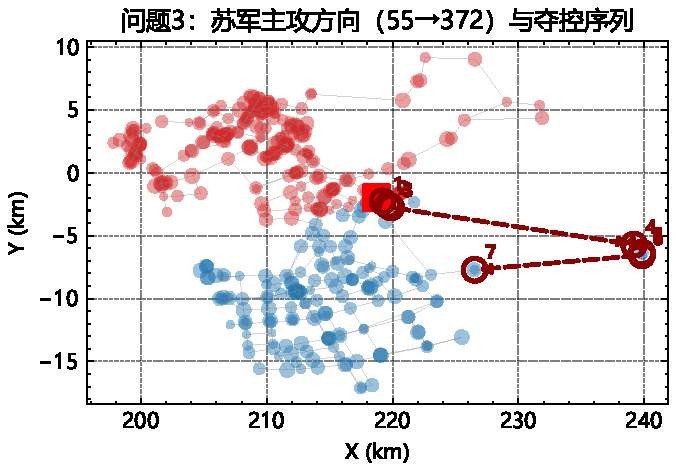
\includegraphics[width=0.46\textwidth]{result_bundle/figures/fig7_attack_plan.pdf}
\caption{问题三苏军主攻方向（55$\to$372）与夺控序列（编号为夺控顺序）}
\label{fig:attack}
\end{figure}

\subsubsection{盟军两情景战略转移模型}

盟军需从各部署节点收缩至目标集 $\mathcal{T}=\{352,144,149\}$。决策量纲为人员（动员兵，万人）：盟军共 100 万人，另有装备 15710 辆/门（折算吨位 126340 吨）。装备随建制伴随转移，即按各目标承接的人员份额比例随迁，属报告口径而非决策量；目标节点的车辆数/吨位容量题目未给出，故不设车辆容量约束，占用强度以人员容量为基准如实报告。通信畅通情景为集中调度：目标节点的人员分配按防御强度与容量加权，
\begin{equation}
\mathrm{alloc}_t=\frac{0.6\,d_t+0.4\,\min(\mathrm{cap}_t,100)/100}{\sum_{t'}\big(0.6\,d_{t'}+0.4\,\min(\mathrm{cap}_{t'},100)/100\big)}\times \text{总人员}
\label{eq:alloc}
\end{equation}
容量 $\mathrm{cap}_t=\deg(t)\times 40$（度数乘以容量系数，单位万人，强制分散，防止把兵力堆进单个高防御节点）。人员口径下三节点总容量 200 万人大于总人员 100 万人，容量约束为松（占用率 50\%），比例分配不触发截断；模型仍保留容量上限断言以应对参数变化。求得分配：352 承接 40.8 万人、144 承接 11.3 万人、149 承接 47.8 万人，三节点容量裕度分别为 39.2、28.7、32.2 万人。殿后部队取总人员的 10\%（10 万人），负责迟滞追击、掩护主力。各部署节点按最短路就近选择目标节点，共 7 条转移路线，平均长度 13.405 km；通信中断情景则退化为各部队独立预案：无全局协调，各部队按预先制定的最近目标节点路线分散转移，且缺乏协同使拦截风险放大 1.3 倍（上限 0.6）。

生存概率用蒙特卡洛仿真估计，两情景各 2000 次、种子 2026，按人员加权（权重为各部署节点动员兵万人占比，即所求为人员生存概率）。每次仿真中，每支部队沿路径逐边做伯努利拦截抽样，被拦截损失该段纵队人员的 40\%；畅通情景另有 8\% 的协同加成（错峰出发降低暴露）；整体生存概率为各纵队存活率的人员加权平均。结果：
\begin{equation}
P_{surv}^{\text{畅通}}=0.7956,\qquad P_{surv}^{\text{中断}}=0.6730,\qquad \Delta=0.1226
\label{eq:surv}
\end{equation}

图~\ref{fig:surv} 以带 95\% 置信区间误差棒的柱状图对比两情景。畅通情景均值 0.7956（95\% CI $[0.5962,1.0000]$），中断情景 0.6730（95\% CI $[0.4809,0.8640]$），均值差 0.1226 远大于两情景均值估计的标准误（SEM/mean 为 0.29\% 与 0.32\%），差异在统计上明确。

置信区间较宽是生存率分布双峰性的体现：单次仿真要么大部分部队安全通过、要么在关键边被拦截，样本内在离散大（std/mean 为 12.78\% 与 14.47\%，按阈值判“not converged”），但均值估计本身已收敛，两口径的区分与问题二同理。0.1226 的生存概率差就是“通信的生存价值”的量化：保持通信、集中调度、错峰出发，能让约八分之一的人员免于损失。

\begin{figure}[H]
\centering
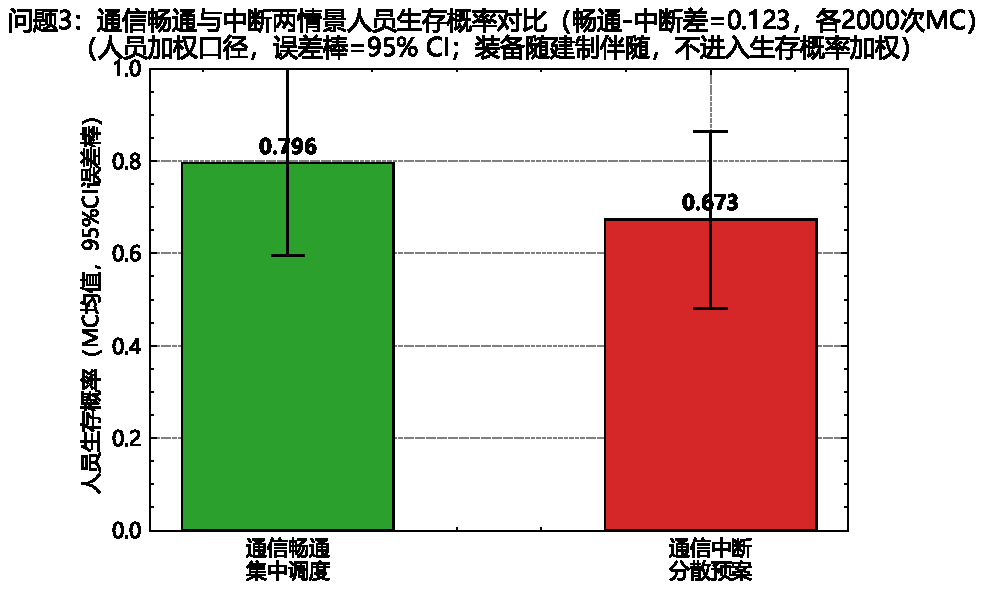
\includegraphics[width=0.46\textwidth]{result_bundle/figures/fig8_survival_comparison.pdf}
\caption{问题三盟军转移人员生存概率对比（人员加权，MC 均值，95\% 置信区间误差棒，各 2000 次仿真）}
\label{fig:surv}
\end{figure}

% ============================================================
% 六、灵敏度与误差分析
% ============================================================
\section{灵敏度与误差分析}
\label{sec:sens}

\subsection{问题一：权重扰动与假设参数化扫描}

对目标权重做 $\pm20\%$ 扰动（扰动后重新归一化），逐扰动向量重解指挥节点评估：苏军 6 组扰动下主选节点 136 翻转 0 次，$\varphi$ 介于 0.7372（$w_3+20\%$）与 0.8034（$w_3-20\%$）之间；盟军节点 384 翻转 0 次，$\varphi$ 介于 0.7418 与 0.8073 之间。权重变化改变效能数值但不改变选址结论，方案对目标权重稳健。

假设 A-02 至 A-04 的参数化扫描结果见表~\ref{tab:sweep}，对应扫描图见图~\ref{fig:sweeps}（自左至右：A-02 直射距离、A-03 防空半径、A-04 空中上限）。

\begin{table}[H]
\centering
\caption{假设参数化扫描的稳定性结论}
\label{tab:sweep}
\zihao{5}
\resizebox{\textwidth}{!}{
\begin{tabular}{p{2.6cm}p{2.6cm}p{4.6cm}p{7.2cm}}
\toprule
参数 & 扫描范围 & 稳定性判据 & 结果 \\
\midrule
A-02 直射距离 $d$ & 1.0--3.0 km，5 点 & 指挥节点不翻转且部署 Jaccard 相似度不低于 0.8 & 双方翻转计数 0，相似度恒为 1.0，$\varphi$ 不变（苏 0.76879、盟 0.77324） \\
A-03 防空半径 $r$ & 2.0--4.0 km，5 点 & 防空节点集 Jaccard 相似度不低于 0.8 & 双方节点变化数为 0，相似度恒为 1.0；含防空口径 $\varphi$ 苏 0.82465、盟 0.82962 \\
A-04 空中上限 $\alpha$ & 5\%--20\%，4 点 & 指挥节点不翻转 & 双方翻转计数 0；空中部署随上限单调不减（$\alpha=20\%$ 时苏军增至 344、386 两节点，Jaccard 0.9744）；经需求传播至 Q2 的成本影响最大 0.419\% \\
\bottomrule
\end{tabular}
}
\end{table}

\begin{figure}[H]
\centering
\begin{minipage}{0.32\textwidth}\centering
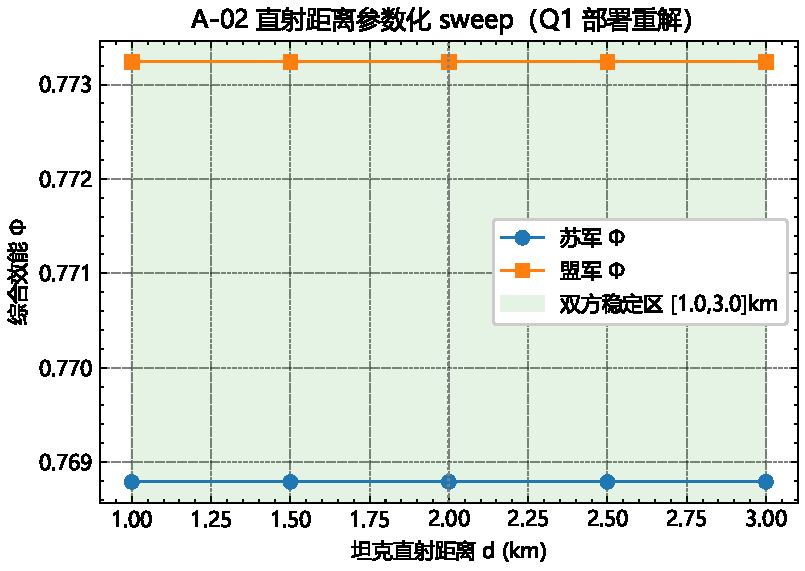
\includegraphics[width=\textwidth]{result_bundle/figures/fig11_q1_direct_range_sweep.pdf}
\end{minipage}\hfill
\begin{minipage}{0.32\textwidth}\centering
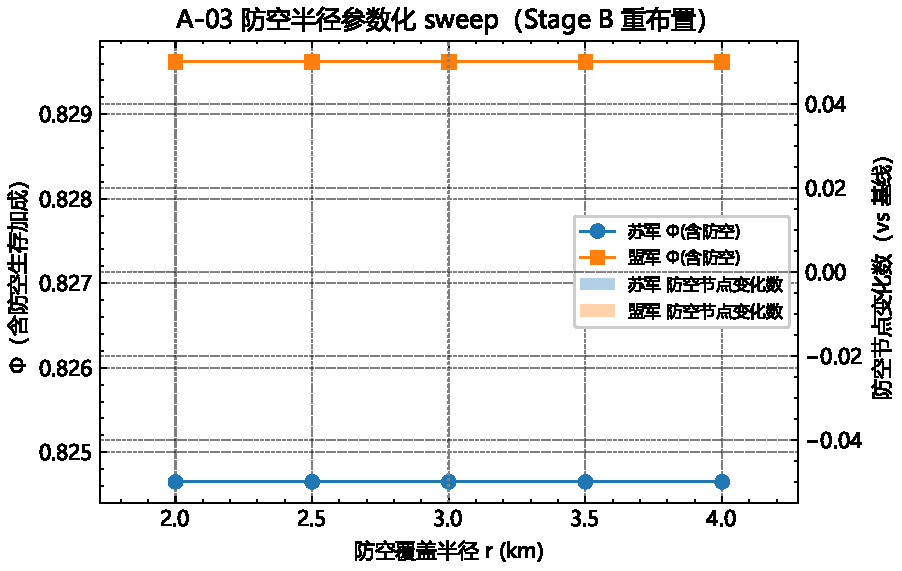
\includegraphics[width=\textwidth]{result_bundle/figures/fig12_q1_aa_radius_sweep.pdf}
\end{minipage}\hfill
\begin{minipage}{0.32\textwidth}\centering
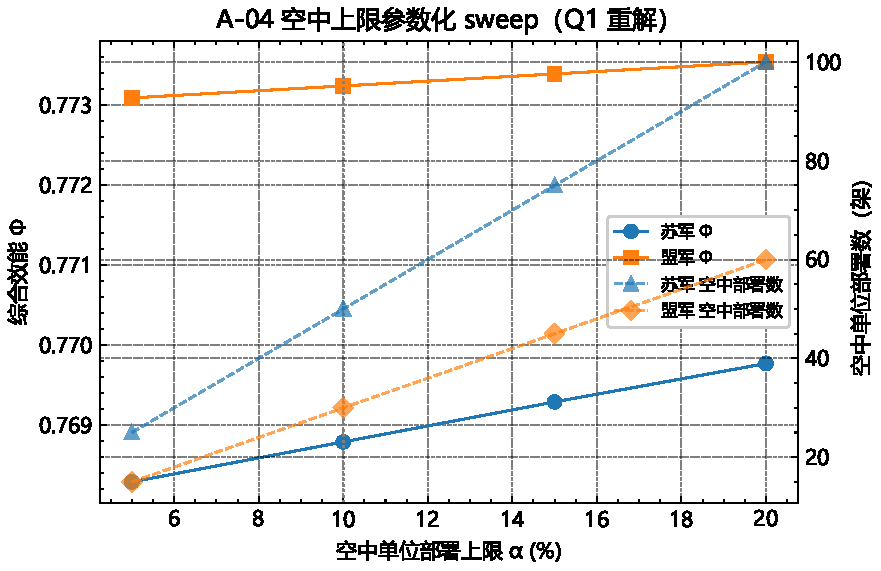
\includegraphics[width=\textwidth]{result_bundle/figures/fig14_q1_air_cap_sweep.pdf}
\end{minipage}
\caption{问题一假设参数化扫描（左：A-02 直射距离 $d\in[1.0,3.0]$ km；中：A-03 防空半径 $r\in[2.0,4.0]$ km；右：A-04 空中上限 $\alpha\in[5\%,20\%]$；纵轴为综合效能）}
\label{fig:sweeps}
\end{figure}

图~\ref{fig:sweeps} 左图中，直射距离从 1.0 km 放大到 3.0 km，双方 $\varphi$ 曲线完全水平（苏军 0.76879、盟军 0.77324），指挥节点与部署结构逐点相同。这一“超稳健”现象的机理是：战场咽喉覆盖约束由火炮（射程 13--16.8 km）主导，坦克直射距离只影响贴近咽喉的少量覆盖关系，在当前部署下不构成瓶颈。它同时给出一个实用结论：即便指挥员对坦克直射距离的估计偏差达 $\pm50\%$，问题一的部署方案无需调整。

\begin{sloppypar}
图~\ref{fig:sweeps} 中图中，防空半径变化同样不改变防空据点布局（10 个据点逐点不变），只有覆盖到的部署节点数随半径单调增加（苏军 140$\to$197、盟军 77$\to$116），生存加成 $S_{bonus}$ 与含防空效能保持常数（苏军 803.5、$\varphi=0.82465$；盟军 1559.4、$\varphi=0.82962$）。原因是据点直接设在部署节点上，半径只要不小于部署节点间距的下限就能覆盖同样的兵力，2.0 km 已满足。
\end{sloppypar}

\begin{sloppypar}
图~\ref{fig:sweeps} 右图中，$\varphi$ 随 $\alpha$ 单调缓升（苏军 0.76829$\to$0.76977、盟军 0.77309$\to$0.77354），空中部署量随上限单调不减：苏军在 $\alpha=5\%$--15\% 时集中部署于 386（25/50/75 架），$\alpha=20\%$ 时扩至 344 与 386 两节点（100 架）；盟军始终集中于 384。“空中单位少量集中部署”的定性结论在全区间稳定，且 $\alpha$ 经部署、需求传播到问题二补给成本的最大影响仅 0.419\%，跨问题传播可忽略。
\end{sloppypar}

\subsection{问题二：成本灵敏度与护航策略临界点}
\label{sec:tornado}

对问题二三类核心参数做缩放扫描：破交概率 $\times0.5$--1.5（10 点）、需求率 $\pm20\%$（6 点）、车载容量 $\pm20\%$（6 点），每次重解 MIP。Tornado 图（图~\ref{fig:tornado}）按 $\pm20\%$ 扰动引起的 TC 变化幅度排序。

\begin{figure}[H]
\centering
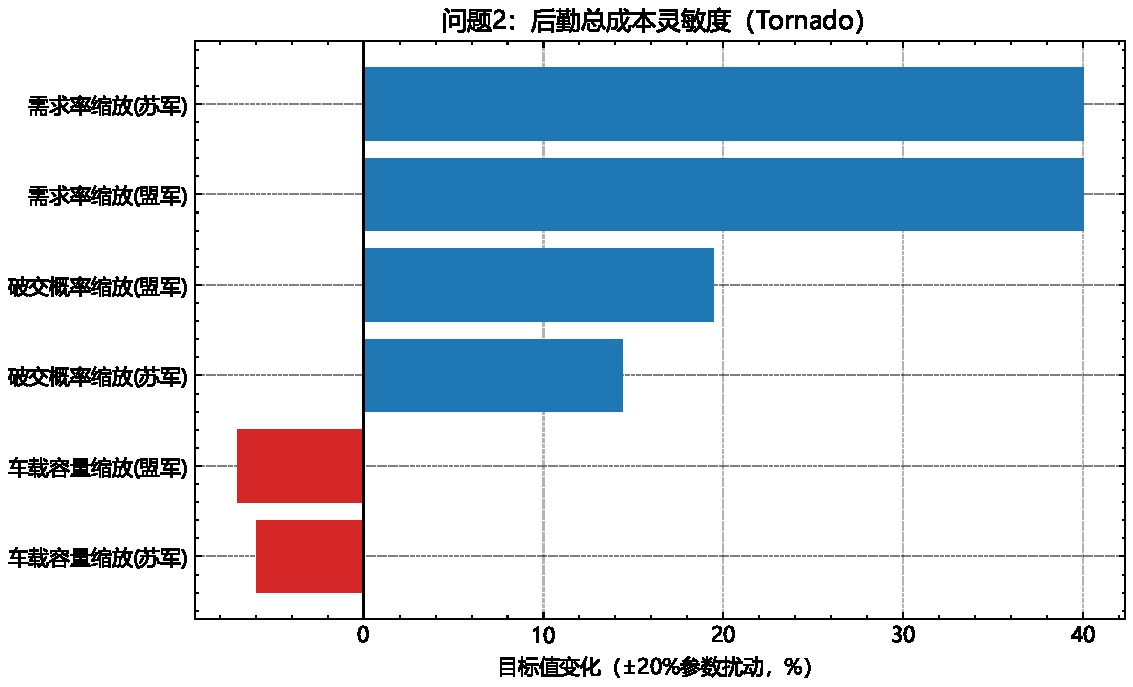
\includegraphics[width=0.46\textwidth]{result_bundle/figures/fig5_tornado_q2.pdf}
\caption{问题二后勤总成本灵敏度 Tornado 图（$\pm20\%$ 参数扰动，基线为不含人力成本口径）}
\label{fig:tornado}
\end{figure}

排序结果为：需求率最敏感，TC 随需求线性响应（$\pm20\%$ 扰动对应 $\mp20\%$ 的 TC 变化，苏军 70411--105617 元/日）；破交概率次之且不对称，风险减半（$\times0.5$）使苏军 TC 下降 27.02\%、盟军下降 31.46\%，风险加倍（$\times1.5$）仅上升 12.18\% 与 18.87\%，因为高风险下路径选择会绕行避险，边际损失递减；车载容量影响最弱（$\pm20\%$ 对应 $\mp2.4\%$--3.6\%），容量只改变车次数，不改变路径结构。本扫描以不含人力成本口径计算：人力成本由车辆数与装卸量决定，占比约两成且不改变上述敏感度排序；正文主结论一律以含人力 $\mathrm{TC}_{total}$ 口径报告，两口径可据表~\ref{tab:q2cost} 互相换算。管理含义明确：降低前线需求（精简携行标准、就地筹措）对节约后勤成本的杠杆最大，其次是压制敌方破交能力。

\begin{figure}[H]
\centering
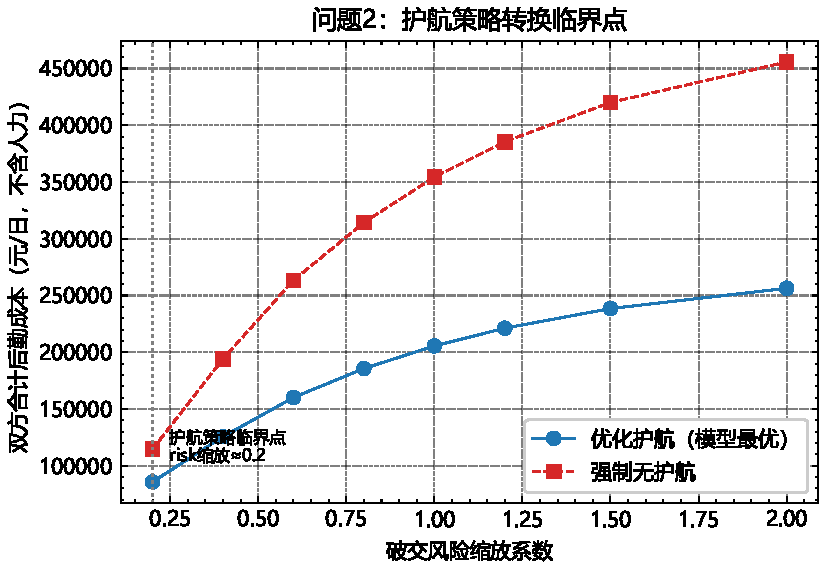
\includegraphics[width=0.46\textwidth]{result_bundle/figures/fig6_escort_critical.pdf}
\caption{问题二护航策略转换临界点（横轴为破交风险缩放系数，纵轴为双方合计后勤成本，不含人力）}
\label{fig:escort}
\end{figure}

\begin{sloppypar}
护航是否为必需投入，用策略转换临界点回答。对风险缩放系数 $s\in\{0.2,0.4,\dots,2.0\}$，分别求解“自由护航”与“强制无护航”两个方案并对比总成本（图~\ref{fig:escort}，不含人力成本口径）。自由护航方案的 TC 从 $s=0.2$ 的 85758 元/日单调升至 $s=2.0$ 的 256358 元/日；强制无护航方案从 114603 升至 455800，始终在上方。扫描区间内自由护航恒优，临界风险缩放为 0.2（扫描下限），即只有当真实风险低于基线估计的 20\% 时护航才不经济。基线 $s=1.0$ 深处护航区：无护航将使双方合计成本从 205587 升至 354259 元/日，增幅 72.3\%。人力成本由车辆数与装卸量决定、与是否启用护航无关，若两方案同加基线人力成本 49800 元/日（苏军 21600、盟军 28200），方案差不变，护航恒优的定性结论不受口径影响。可见护航不是可选项，而是当前风险环境下的必需项。
\end{sloppypar}

活跃约束方面，问题二全部 10 个需求约束均紧（各需求节点流入恰等于需求，无过量补给），派生量即各节点需求值（如苏军节点 386 为 28.76 吨/日、盟军节点 384 为 45.68 吨/日），说明最优方案按需精确配送，没有冗余运力。

\subsection{问题三：主攻方向翻转条件与风险敏感性}
\label{sec:flip}

主攻边 55$\to$372 与次优边 251$\to$166 的评分差仅 0.0227，有必要给出翻转的定量条件。把式~\eqref{eq:axis} 按项分解：次优边敌方端点防御更弱（0.45 对 0.58），防御项领先 $0.5\times(0.58-0.45)=0.065$；但其纵深项低 0.0377，两项合计次优边在非走廊项上仍领先 0.0273。主攻边的优势全部来自走廊价值（端点度数归一值 0.5 对 0.3333，按权重 0.3 折算领先 0.05）。

据此得到两个翻转条件。其一，走廊权重由 0.3 下调至 0.1638（降幅 45.4\%）时次优边反超；上调走廊权重只会拉大差距，因为主攻边的走廊价值更高。其二，主攻边敌方端点防御强度的估计值上调 0.0454（由 0.58 至 0.6254）时，防御项得分下降 0.0227，两边打平，再高则次优边反超。评分差小意味着主攻方向处于参数敏感区：防御情报只要偏差 0.045 就足以改变结论，指挥员若掌握更精确的敌防御估计，应重算评分再定案；在现有情报精度下，55$\to$372 仍是评分最优。以上阈值由评分公式直接解出，与代码重算一致。

盟军转移的拦截风险敏感性见图~\ref{fig:q3sens}：风险缩放系数从 0.8 到 1.2，畅通情景人员生存概率从 0.8466 单调降至 0.7506，中断情景从 0.7314 降至 0.6248。两条曲线在整个扫描区间内不相交，即不存在情景翻转临界点：无论风险估计偏高还是偏低 20\%，集中调度都优于分散预案，0.1226 的生存差结论对风险参数稳健。

\begin{figure}[H]
\centering
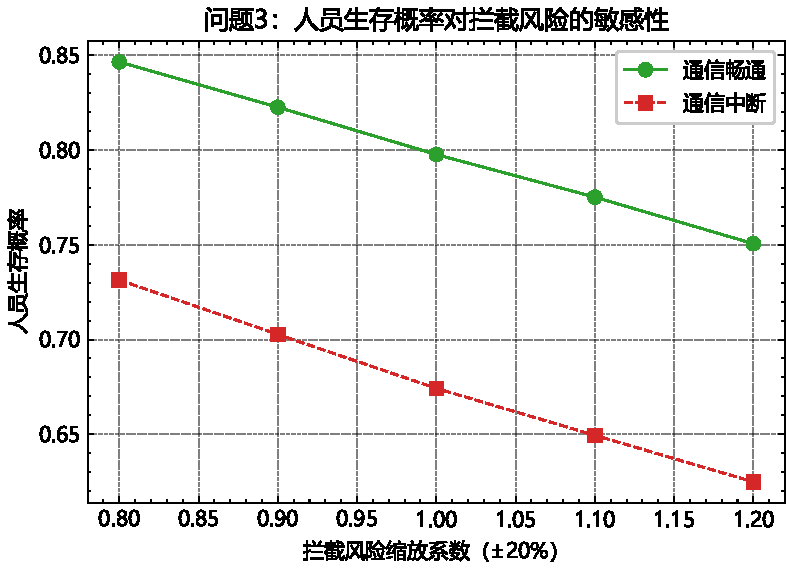
\includegraphics[width=0.46\textwidth]{result_bundle/figures/fig10_q3_risk_sensitivity.pdf}
\caption{问题三人员生存概率对拦截风险的敏感性（人员加权，$\pm20\%$ 缩放，两情景各 1000 次仿真）}
\label{fig:q3sens}
\end{figure}

\subsection{误差来源、量化与可接受性}
\label{sec:err}

\textbf{（1）护航成本线性化近似}。MIP 内部目标值与重算 TC 的差距为苏军 7.18\%、盟军 8.56\%（以不含人力成本口径 88013.7 与 117573.0 为分母），来源是护航成本按需求均分份额线性化，与真实“车次数$\times$单次护航费”存在偏差。该近似只影响求解时的目标引导，不影响方案可行性：最终报告的 TC 是对 MIP 解的逐项重算真值，偏差方向与幅度已知、可接受。

\textbf{（2）破交概率公式假设}。$\mathrm{risk}_e$ 以边度数与跨阵营属性代理暴露程度，属内生未知参数（A-01）。其影响通过两条通道量化：蒙特卡洛模型验证偏差 0.72\% 与 1.54\%（公式期望与伯努利仿真一致，说明公式内部自洽）；Stackelberg 最坏情形给出对抗上限 $+50.83\%/+48.94\%$（含人力 $\mathrm{TC}_{total}$ 主口径）。两者夹住了基线估计的误差带。

\textbf{（3）守军强度标定}。$k_{def}=0.5+0.3\,d$ 是线性粗标定：防御 0.89 的节点守军仅为攻方投入的 0.767 倍，这使各步胜率偏高（0.982--1.000）、剩余比偏高（0.845--0.912）。真实防御还依赖工事、预备队与火力配系，线性标定无法刻画。该局限的边界是：夺控序列的相对排序（先易后难）与可行性不受影响，但胜率的绝对数值应视为乐观估计，投入实战规划时需按更保守的标定重算。

\textbf{（4）决策粒度}。动员兵万人粒度相对 0.5 万人细粒度的效能差为 0.0001（苏军）与 0.00001（盟军），部署结构 Jaccard 为 1.0，粒度误差可忽略。

\textbf{（5）蒙特卡洛估计误差}。问题三人员生存概率的 SEM/mean 为 0.29\%（畅通）与 0.32\%（中断），2000 次仿真下均值估计的抽样误差远小于两情景差 0.1226；问题二损失仿真以均值偏差 0.72\%/1.54\% 为收敛判据。std/mean 超阈值（12.78\%、14.47\%、46.70\%、54.61\%）均为复合分布内在离散所致，不代表估计未收敛，两处均已双口径披露。

\textbf{（6）路径截断与行程约束简化}。每对起讫点保留 3 条候选路径，扩到 5 条后 TC 改善为 0.0\%（双方均无改善），截断合理。问题一忽略行程对部署的约束：最紧的天启坦克行程一半为 90 km，大于战场直径 43.3 km，该约束恒不活跃，简化差异为 0。

\textbf{鲁棒性小结}。问题一的部署与选址在权重 $\pm20\%$、直射距离 $[1.0,3.0]$ km、防空半径 $[2.0,4.0]$ km、空中上限 $[5\%,20\%]$ 内全部稳定；问题二的护航策略在风险缩放 $[0.2,2.0]$ 内恒优、需求线性响应可预测；问题三的情景排序在风险 $\pm20\%$ 内无交叉。三个问题的核心结论对各自的关键不确定参数均稳健。

% ============================================================
% 七、模型评价与推广
% ============================================================
\section{模型评价与推广}

\subsection{优势}

其一，结构线性化换取可证明的最优性：覆盖边际递减、护航—损失耦合两处非线性分别以有效覆盖变量与 McCormick 线性化精确处理，问题一、问题二全部实例由分支定界证明全局最优（MIPGap=0），求解时间在 0.4 s 以内。其二，图结构驱动的建模简化均有数值验证支撑：坐标单位核验（比值恒 1.0000）免去路网距离预计算，行程约束恒不活跃、路径截断改善为 0 两项对比证明了简化的无损性。其三，成本四分层与显式参数化使结论可归因、假设可检验：破交损失主导（68.8\%/67.1\%）直接指向“压制破交”这一管理抓手，A-01 至 A-04 全部给出稳定性区间或最坏情形量化。

\subsection{局限性}

其一，$k_{def}=0.5+0.3\,d$ 的守军标定粗糙，夺控胜率（0.982--1.000）与剩余比（0.845--0.912）偏乐观，进攻方案的绝对消耗估计可信度低于其相对排序。其二，$\mathrm{risk}_e$ 为静态公式，Stackelberg 最坏情形是事后对照而非嵌入求解的双层均衡，方案在对抗意义下只是领导者单方可行的稳健解。其三，进攻序列为贪心构造，无全局最优保证；动员兵万人粒度的验证只证明了结构稳健，未证明细粒度下无更优解。

\subsection{改进方向与推广}

改进方向有三：把问题二扩展为双层规划，将敌方最优响应内嵌求解以得到真正的 Stackelberg 均衡方案；引入需求波动与战损下的滚动时域动态重调度；将问题三的贪心升级为走廊子图（约 30 节点）上的时序 MIP，量化最优性差距。模型框架可推广到一般“部署—补给—机动”三层运筹问题：覆盖型指派适用于防空布防与传感器布置，成本分层加对抗最坏情形适用于航运护航与供应链中断管理，两情景生存仿真适用于应急疏散的通信保障评估。

\subsection{题目设计合理性讨论}

题目设计总体合理且富有区分度，三点具体讨论。其一，参数缺口：附件二提供了自行火炮最大射程，但未提供任何坦克的直射距离与防空炮覆盖半径，而问题一明确要求考虑这两类射程，建模者只能以假设补足（A-02、A-03），建议题目后续版本补充该数据或给出标定指引。其二，粒度失配：动员兵以百万计（125 万、100 万），与 436 节点的战场粒度失配，题目未提示聚合方式，建模者需自行决定决策粒度（本文取万人并附验证），属设计粗糙处。

其三，非对称对抗设计良好：苏军射程优势（V3 16.8 km 对光棱 13.0 km）与盟军数量优势（火炮 14000 对 7000）形成互补性对抗，模型自然涌现出“数量优势不等于后勤优势”（盟军 TC 高 33.0\%）等可讨论的结论，说明题目参数能支撑有深度的分析。

% ============================================================
% 参考文献
% ============================================================
\newpage
\begin{thebibliography}{99}
\zihao{5}
\bibitem{ref1} 姜启源, 谢金星, 叶俊. 数学模型[M]. 5版. 北京: 高等教育出版社, 2018.
\bibitem{ref2} 钱颂迪. 运筹学[M]. 4版. 北京: 清华大学出版社, 2012.
\bibitem{ref3} SCHRIJVER A. Combinatorial Optimization: Polyhedra and Efficiency[M]. Berlin: Springer, 2003.
\bibitem{ref4} WOLSEY L A. Integer Programming[M]. New York: Wiley, 1998.
\bibitem{ref5} DIJKSTRA E W. A note on two problems in connexion with graphs[J]. Numerische Mathematik, 1959, 1(1): 269-271.
\bibitem{ref6} YEN J Y. Finding the $k$ shortest loopless paths in a network[J]. Management Science, 1971, 17(11): 712-716.
\bibitem{ref7} MCCORMICK G P. Computability of global solutions to factorable nonconvex programs: Part I — Convex underestimating properties[J]. Mathematical Programming, 1976, 10(1): 147-175.
\bibitem{ref8} LANCHESTER F W. Aircraft in warfare: The dawn of the fourth arm[M]. London: Constable and Company, 1916.
\bibitem{ref9} BRACKEN J. Lanchester models of warfare[J]. European Journal of Operational Research, 1983, 14(1): 59-65.
\bibitem{ref10} BASAR T, OLSDER G J. Dynamic Noncooperative Game Theory[M]. 2nd ed. Philadelphia: SIAM, 1999.
\bibitem{ref11} RUBINSTEIN R Y, KROESE D P. Simulation and the Monte Carlo Method[M]. 3rd ed. Hoboken: Wiley, 2016.
\bibitem{ref12} TAYLOR J G. Lanchester-type models of combat[J]. Journal of Mathematical Analysis and Applications, 1983, 96(2): 429-444.
\end{thebibliography}

% ============================================================
% 附录
% ============================================================
\appendix
\sloppy  % 附录含长文件路径，允许宽松断行避免溢出

\section{支撑材料文件列表}

支撑材料包含以下文件，与论文结论一一对应：

\begin{enumerate}[label=(\arabic*),leftmargin=2em,itemsep=0.2em]
\zihao{5}
\item 源程序：project/ 下 11 个 Python 脚本——common\_data.py、solver\_backend.py、visualization\_style.py、data\_explore.py、geometry\_check.py、问题1\_求解.py、问题2\_求解.py、问题3\_求解.py、验证分析.py、参数化扫描.py、图表生成.py（全部代码亦见下节，与运行版本逐行一致）；
\item 数据文件：project/data/ 下附件一：作战节点与通路数据.xlsx（节点与通路两个工作表）、附件二：红警装备参数表.xlsx（赛题原始数据，随包提供以保证程序可直接运行）；
\item 图表文件：project/figures/ 下 fig1 至 fig14 共 14 张图（PDF 与 PNG 双格式）。
\end{enumerate}

运行说明：按附录所列执行顺序依次运行各脚本即可复现全部结果；各脚本运行时在 project/results/ 下生成中间结果文件，供后续脚本与图表生成读取。

\section{完整可运行源程序代码}

以下代码为建模与求解的全部源程序，按执行顺序排列，均以 VerbatimInput 直接引用 project/ 目录下的实际源文件，与运行代码逐行一致（含中文注释）。运行环境为 Python 3，依赖 numpy、pandas、pulp、matplotlib；求解器为 pulp 自带的 CBC/HiGHS 开源后端。执行顺序：data\_explore.py（数据剖析）$\to$ geometry\_check.py（几何核验）$\to$ 问题1\_求解.py $\to$ 问题2\_求解.py $\to$ 问题3\_求解.py $\to$ 验证分析.py $\to$ 参数化扫描.py $\to$ 图表生成.py；common\_data.py 为共享数据层，solver\_backend.py 为统一求解后端，visualization\_style.py 为统一图表样式。

\subsection{common\_data.py（共享数据层：图加载、最短路、风险计算）}
\VerbatimInput{project/common_data.py}

\subsection{solver\_backend.py（统一 MIP/LP 求解后端）}
\VerbatimInput{project/solver_backend.py}

\subsection{visualization\_style.py（统一图表样式）}
\VerbatimInput{project/visualization_style.py}

\subsection{data\_explore.py（附件数据剖析）}
\VerbatimInput{project/data_explore.py}

\subsection{geometry\_check.py（几何核验与连通性分析）}
\VerbatimInput{project/geometry_check.py}

\subsection{问题1\_求解.py（部署优化与指挥节点选址）}
\VerbatimInput{project/问题1_求解.py}

\subsection{问题2\_求解.py（补给网络优化与 Stackelberg 最坏情形）}
\VerbatimInput{project/问题2_求解.py}

\subsection{问题3\_求解.py（进攻方案与两情景转移仿真）}
\VerbatimInput{project/问题3_求解.py}

\subsection{验证分析.py（灵敏度、临界点、蒙特卡洛模型验证）}
\VerbatimInput{project/验证分析.py}

\subsection{参数化扫描.py（假设 A-01 至 A-04 参数化扫描与粒度验证）}
\VerbatimInput{project/参数化扫描.py}

\subsection{图表生成.py（全部 14 张图表）}
\VerbatimInput{project/图表生成.py}

\end{document}
